\documentclass[a4paper,fleqn]{cas-dc}

\usepackage[authoryear,longnamesfirst]{natbib}
\usepackage{microtype}
\usepackage{amsthm}
\usepackage{booktabs}
\usepackage{placeins}
\usepackage{dsfont}
\usepackage[nameinlink,capitalise]{cleveref}

\usepackage{nicefrac}


\newtheorem{theorem}{Theorem}
\newtheorem{lemma}{Lemma}
\newtheorem{proposition}{Proposition}
\newtheorem{corollary}{Corollary}
\theoremstyle{definition}
\newtheorem{definition}{Definition}
\theoremstyle{remark}
\newtheorem{remark}{Remark}

\newcommand{\R}{\mathds{R}}
\newcommand{\N}{\mathds{N}}
\newcommand{\Nzero}{\mathds{N}_0}
\newcommand{\Pp}{\mathds{P}}
\newcommand{\E}{\mathds{E}}
\newcommand{\norm}[1]{\left\lVert #1\right\rVert}
\newcommand{\set}[1]{\left\{#1\right\}}
\newcommand{\dd}{\,\mathrm{d}}
\newcommand{\Leb}{\lambda}
\newcommand{\ellpq}{\ell_{p,q}}
\newcommand{\upq}{u_{p,q}}
\newcommand{\kappaN}[1]{\kappa_{#1}}
\newcommand{\0}{\mathbf{0}}
\newcommand{\spherearea}[1]{\sigma_{#1}}
\newcommand{\tr}[1]{\textcolor[HTML]{aa0000}{#1}}
\newcommand{\tb}[1]{\textcolor[HTML]{0000bb}{#1}}
\newcommand{\ta}[1]{\textcolor[HTML]{99007d}{#1}}
\newcommand{\tg}[1]{\textcolor[HTML]{009999}{#1}}
\DeclareMathOperator{\SSG}{SSG}
\DeclareMathOperator{\RNG}{RNG}
\DeclareMathOperator{\GG}{GG}
\DeclareMathOperator{\Del}{Del}
\DeclareMathOperator{\MST}{MST}
\DeclareMathOperator{\G}{G}

\ExplSyntaxOn
\bool_gset_true:N \g_stm_nologo_bool
\ExplSyntaxOff


\emergencystretch=1em

\begin{document}
\let\WriteBookmarks\relax
\def\floatpagepagefraction{1}
\def\textpagefraction{.001}

\shorttitle{Stepping-Stone Diversion Neighborhoods}
\shortauthors{H. Espino-Montelongo and H. Maravillo}

\title[mode=title]{Geometry and Volume of Stepping-Stone Diversion Neighborhoods in Euclidean Spaces of Arbitrary Dimension}

\author[1]{Heriberto Espino-Montelongo}
    [orcid=0009-0009-1230-2931]
\cormark[1]
\ead{heriberto.espinomo@udlap.mx}
\credit{
  Conceptualization,
  Methodology,
  Formal analysis,
  Investigation,
  Validation,
  Visualization,
  Writing -- original draft}

\affiliation[1]{
  organization={Universidad de las Am\'ericas Puebla},
  addressline={Ex Hacienda Santa Catarina M\'artir S/N},
  city={San Andr\'es Cholula},
  postcode={72810},
  state={Puebla},
  country={Mexico}
}

\author[2]{H\'ector Maravillo}
    [orcid=0000-0002-6101-1964]
\ead{hector.maravillo@uacm.edu.mx}
\credit{
  Investigation,
  Supervision,
  Visualization,
  Writing -- review and editing}

\affiliation[2]{
  organization={Universidad Aut\'onoma de la Ciudad de M\'exico},
  city={Ciudad de M\'exico},
  postcode={06720},
  country={Mexico}
}

\cortext[cor1]{Corresponding author}


\begin{abstract}
The stepping-stone graph forms a one-parameter family of empty-region graphs originally introduced in the plane.
We develop a geometric, graph-theoretic, and % Agregue esta porque tambien creo que es importante hablar del SS graph
probabilistic analysis of the stepping-stone graph in
\(\R^d\), for every \(d\geq2\).
 % 
The volume of the diversion neighborhood 
factorizes as the \(d\)th power of
the distance between the defining sites times a 
normalized constant that depends only on $\alpha$, 
the stepping-stone parameter.
% sisa >:D
An explicit boundary parametrization reduces
the original \(d\)-dimensional volume problem to a one-dimensional integral.
We recover the degenerate case and the case corresponding to the region
defining the Gabriel graph
and prove, in every dimension,
that, after removing the two defining sites, the finite-parameter
neighborhoods converge from within to 
the open lune defining the relative-neighborhood
graph. % para que quede igual que el de gg
Consequently, their volumes converge to the classical % unit-lune % creo que es mejor decir que converge solo al volumen, por la prorposicion 1
volume of the lune defining the 
relative-neighborhood graph, for which we record an equivalent regularized
incomplete-beta representation. For arbitrary ambient dimension, we also
prove strict region and volume monotonicity, derive the
corresponding inclusions among classical proximity graphs, establish
connectivity, and show that, for $\alpha\geq2$, the defining empty-region
condition need only be evaluated for 
those edges in the Gabriel graph 
that are not in the open relative-neighborhood graph. %open-lune relative-neighborhood edges. 
The resulting volume constant specializes
existing expected-size results for random proximity graphs. Finally, a
 change of variables gives a stable quadrature formula, 
 which we validate independently
by rejection sampling applied directly to the
defining inequality.

\end{abstract}

\begin{keywords}
Stepping-stone graph \sep empty-region graph \sep proximity graph \sep volume constant \sep stochastic geometry \sep computational geometry
\end{keywords}

\maketitle

\hypersetup{
  pdftitle={
    Geometry and Volume of Stepping-Stone Diversion Neighborhoods
    in Euclidean Spaces of Arbitrary Dimension
  },
  pdfauthor={
    Heriberto Espino-Montelongo and Héctor Maravillo
  },
  pdfkeywords={
    stepping-stone graph,
    empty-region graph,
    proximity graph,
    volume constant,
    stochastic geometry,
    computational geometry
  }
}

\section{Introduction}
An empty-region proximity graph joins two sites whenever a region
determined by them contains no other site. Classical examples include
the Gabriel graph, the relative-neighborhood graph, and the
$\beta$-skeletons
\citep{gabriel1969statistical,toussaint1980relative,
jaromczyk1992relative,kirkpatrick1985framework}.
The theoretical, probabilistic, and algorithmic properties of proximity
graphs have been extensively studied
\citep{bose2013spanners,devroye1988expected,cardinal2009empty}.
Higher-dimensional proximity constructions include
relative-neighborhood graphs in $\R^3$~\citep{agarwal1992relative} and
extensions of proximity regions to higher dimensions
\citep{ceyhan2010extension}.
These graphs also have applications in pattern recognition, data analysis,
and spatial-network modeling
\citep{jaromczyk1992relative,watanabe2008evaluating}.

The stepping-stone graph was introduced by
\citet{kannangara2018stepping} for movement analysis and subsequently
developed in
\citep{kannangara2019stepping}. Those works study the parameterized family
of planar proximity graphs obtained as the diversion parameter varies, its
relationship with classical proximity graphs, and its application to
movement-corridor analysis.
The parameter regulates how readily a third site can serve as a
diversion between a pair of sites and hence controls the edges retained by
the graph. We denote their parameter by $\alpha$, reserving $d$ for the
ambient dimension.


In the original formulation,
a planar point belongs to the diversion neighborhood
when the sum of the $\alpha$th powers of its distances to the two defining
sites does not exceed the $\alpha$th power of the distance between the
sites. For a point set $V$, two points $p,q\in V$ are adjacent in the
stepping-stone graph precisely when this neighborhood contains no point of
$V\setminus\{p,q\}$.
The diversion neighborhood reduces to the segment
joining the sites at $\alpha=1$ and equals the region associated with the
Gabriel graph at $\alpha=2$.
It has been shown that the relative-neighborhood graph is the limiting
member of the graph family and that the family is nested under edge inclusion
\citep{kannangara2018stepping,kannangara2019stepping}.
Although the original definition is planar, the same inequality defines a
diversion neighborhood
in $\R^d$ for every $d\geq2$.


The principal contribution of this paper is a unified arbitrary-dimensional
framework for the stepping-stone diversion neighborhood. For every
$d\geq2$, we derive its similarity factorization, obtain an explicit boundary
parametrization and a one-dimensional integral for its normalized volume,
and establish the resulting graph inclusions, connectivity properties,
and probabilistic consequences.
The volume is especially relevant under random-point models, where it enters
empty-region probabilities and the constants governing expected graph size.
To our knowledge, an explicit boundary parametrization and a
dimension-uniform one-dimensional volume representation have not previously
been established for the stepping-stone family.


The main difficulty is that the defining distance condition describes the
region only implicitly. Direct numerical computation therefore treats every
choice of dimension and parameter as a new multidimensional integration
problem over a curved region. We instead place the two sites in a standard
position and exploit the rotational symmetry around the line joining them.
An explicit description of the resulting boundary profile then reduces the
volume calculation to a one-dimensional integral.

The similarity reduction provides a normalization principle. Once the
dimension $d$ and the parameter $\alpha$ are fixed, changing the distance
between the two sites changes only the scale of the diversion neighborhood,
not its normalized shape, so its volume factorizes into the $d$th power of
that distance and a constant depending only on $\alpha$ and $d$. The main
theorem is the analytic reduction from the implicitly defined boundary to an
explicit parametrization and then to a one-dimensional integral for this
constant.

We also derive a numerically stable form for its evaluation and recover the
degenerate segment, the closed ball associated with the Gabriel graph, 
and the relative-neighborhood limit.
We further prove, for every $d\geq2$, that both the diversion neighborhoods
and their volumes increase strictly with $\alpha$, while the corresponding
empty-region graphs decrease under edge inclusion. We establish strict
containment in
the closed ball defining the Gabriel graph
for $1\leq\alpha<2$, obtain dimension-dependent bounds for the normalized
volume constants, and derive connectivity and classical graph inclusions.
These results refine the previously known monotonic decrease of the planar
stepping-stone graphs by establishing strict geometric and volumetric
monotonicity in arbitrary dimension.


We
locate the stepping-stone graph within 
the classical inclusion hierarchy involving the
minimum spanning tree, relative-neighborhood graph, Gabriel graph, and
Delaunay graph, and obtain connectivity in every ambient dimension. 
These inclusions are consequences of the region comparisons. 
For each fixed finite
point set, the nested graph family stabilizes exactly at the open-lune
relative-neighborhood graph after a finite, point-set-dependent parameter.



For diversion-parameter values of two or greater, 
every edge in the stepping-stone graph
must also be an edge in the Gabriel graph, 
whereas every edge in the open-lune relative-neighborhood graph
is automatically retained. Consequently, once the Gabriel and open-lune
relative-neighborhood graphs have been constructed, 
only those edges in the Gabriel graph that are not also edges 
in the relative-neighborhood graph remain undecided and require
evaluation of the stepping-stone empty-region condition. In the plane and
under general position, the Delaunay graph provides a linear-size starting
graph. In higher dimensions, however, 
the inclusions in the Delaunay and Gabriel graphs
do not by themselves provide a subquadratic worst-case starting set.

The relevance of the normalized volume constant is also reflected in
probabilistic analyses of proximity graphs.
Devroye's theorem for graphs defined by regular sets
relates the volume of the normalized empty
region to limiting expected degrees and asymptotic edge-count bounds
\citep{devroye1988expected}. We verify the required regularity conditions for
the stepping-stone graph family and obtain the corresponding asymptotic expected
degree and edge-count lower bound for every $d\geq2$.
In the planar Poisson setting, the same area constant can be used in
Watanabe's edge-length approximation
\citep{watanabe2008evaluating}.
These are applications of existing probabilistic frameworks; the
contribution supplied here is the previously unavailable stepping-stone
volume constant and its geometric derivation in arbitrary dimension.

For numerical evaluation, we derive a change of variables that removes the
endpoint singularity present in the original integral representation. 
% \tb{The
% resulting stable quadrature formula is implemented in the
% \textsc{ProximityGraphs} Python package
% \citep{maravillo2026proximitygraphs}.} % Recomendación eliminar esta oración: En algunos ambitos matemáticos, no hay mucho aprecio a Python, así que recomendaría no hablar de Python en la introducción, dejarlo solo para la sección 6.
% JAJAJA :(
The computational companion to this paper \citep{espino2026computational} records the quadrature,
visualization, and validation procedures, together with their outputs,
sample counts, and deterministic seeds. The numerical values are
independently validated through rejection sampling applied directly to the
defining inequality; this calculation does not use the boundary
parametrization or either quadrature formula.



The remainder of the paper is organized as follows.
\Cref{sec:geometry} defines the normalized diversion neighborhood and
establishes similarity normalization and its elementary geometric
properties.
\Cref{sec:boundary-volume} derives the boundary parametrization and the
one-dimensional volume formula and treats the degenerate case and the cases corresponding to the Gabriel and relative-neighborhood graphs.
\Cref{sec:monotonicity-graphs} proves strict region and volume monotonicity
and records the resulting graph inclusions, connectivity,
finite-parameter stabilization, and candidate-set consequences.
% \Cref{sec:probabilistic-consequences} applies Devroye's expected-size \tb{theory} % Es realmente una teoría, o más bien es un enfoque?
% and presents the planar \tb{restricted-search edge-length approximation.} % es necesario el "restricted-search?. Además no hace falta decir "Section 5 applies Devroye's ... and presents the planar .... [for the stepping stone graphs]? Es decir explicar a que se aplica.
\Cref{sec:probabilistic-consequences} applies Devroye's
theorem for graphs to obtain expected-degree and edge-count
results for the stepping-stone graph. It also specializes Watanabe's
edge-length approximation to the planar stepping-stone family.
Finally, \Cref{sec:numerical} develops the stable quadrature, describes the
computational implementation, and reports the independent numerical validation.


\section{Definitions and geometric preliminaries}
\label{sec:geometry}

Throughout, $d\geq2$ denotes the ambient dimension, and all points and
regions are considered in $\R^d$. 
We write $\0$ for the origin, $e_1$ for the first standard basis vector,
and
\begin{equation}
    B(x,r)
    :=
    \set{z\in\R^d:\norm{z-x}\leq r}
\end{equation}
for the closed Euclidean ball of radius $r$ centered at $x\in\R^d$, and
\begin{equation}
    B^\circ(x,r)
    :=
    \set{z\in\R^d:\norm{z-x}<r}
\end{equation}
for the corresponding open ball.
Furthermore, $\lambda_d$ denotes $d$-dimensional Lebesgue measure, and
\begin{equation}
    \kappa_d
    :=
    \lambda_d\bigl(B(\0,1)\bigr)
    =
    \frac{\pi^{\nicefrac{d}{2}}}{\Gamma(1+\nicefrac{d}{2})}
\end{equation}
is the volume of the unit ball in $\R^d$.

\begin{definition}[Stepping-stone diversion neighborhood]
Let $p,q\in\R^d$ be distinct, and set
\begin{equation}
    \ellpq:=\norm{q-p},
    \qquad
    \upq:=\frac{q-p}{\ellpq}.
\end{equation}
For $\alpha\geq1$, the stepping-stone diversion neighborhood determined by
$p$ and $q$ is
\begin{equation}\label{eq:ss-region}
    S_{\mathrm{SS},\alpha}(p,q)
    :=
    \set{
        z\in\R^d:
        \norm{z-p}^{\alpha}
        +
        \norm{z-q}^{\alpha}
        \leq
        \ellpq^{\alpha}
    }.
\end{equation}


Its normalized region is
\begin{equation}\label{eq:unit-region}
    K_{\mathrm{SS},\alpha}
    :=
    S_{\mathrm{SS},\alpha}(\0,e_1)
    =
    \set{
        z\in\R^d:
        \norm{z}^{\alpha}
        +
        \norm{z-e_1}^{\alpha}
        \leq1
    }.
\end{equation}
\end{definition}


The normalized volume constant is
\begin{equation}
    a_{d,\mathrm{SS}}(\alpha)
    :=
    \lambda_d\bigl(K_{\mathrm{SS},\alpha}\bigr).
\end{equation}


Following the standard terminology for empty-region graphs
\citep{devroye1988expected,cardinal2009empty}, we use the following
arbitrary-dimensional formulation.

\begin{definition}[Empty-region graph]
Let $V\subset\R^d$ be finite or locally finite, and let $N$ be a symmetric
region assignment that associates with every pair of distinct points
$p,q\in\R^d$ a region
\begin{equation}
N(p,q)=N(q,p)\subseteq\R^d.
\end{equation}
The empty-region graph induced by $N$ on $V$ is the simple undirected graph
\begin{equation}
\G_N(V):=\bigl(V,E_N(V)\bigr),
\end{equation}
where $V$ is the vertex set and $E_N(V)$ is the edge set defined by
\begin{equation}
\{p,q\}\in E_N(V)
\quad\Longleftrightarrow\quad
N(p,q)\cap\bigl(V\setminus\{p,q\}\bigr)=\varnothing
\end{equation}
for every pair of distinct vertices $p,q\in V$. For brevity, we write
$ pq\in E_N(V)$ to mean $\{p,q\}\in E_N(V)$.
\end{definition}

For later comparison, let $p,q\in\R^d$ be distinct. The closed and open
regions defining the corresponding Gabriel graphs are the closed and open
balls with diameter $pq$, respectively
\citep{gabriel1969statistical,matula1980properties}:
\begin{eqnarray}
G_{\mathrm{cl}}(p,q)
&:=&
B\!\left(\frac{p+q}{2},\frac{\ellpq}{2}\right),\\
G_{\mathrm{op}}(p,q)
&:=&
B^\circ\!\left(\frac{p+q}{2},\frac{\ellpq}{2}\right).
\end{eqnarray}

The closed and open regions defining the corresponding
relative-neighborhood graphs are
\citep{toussaint1980relative,jaromczyk1992relative}
\begin{eqnarray}
L_{\mathrm{cl}}(p,q)
&:=&
B(p,\ellpq)\cap B(q,\ellpq),\\
L_{\mathrm{op}}(p,q)
&:=&
B^\circ(p,\ellpq)\cap B^\circ(q,\ellpq).
\end{eqnarray}

Henceforth, we refer to $G_{\mathrm{cl}}(p,q)$ and
$G_{\mathrm{op}}(p,q)$ as the closed and open Gabriel balls, respectively,
and to $L_{\mathrm{cl}}(p,q)$ and $L_{\mathrm{op}}(p,q)$ as the closed and
open relative-neighborhood lunes, respectively. 
% \tb{This explicit open--closed
% distinction records the boundary conventions used in the empty-region
% literature and in the original stepping-stone construction
% \citep{cardinal2009empty,kannangara2018stepping}.} % Es necesaria esta precisión?
The associated
empty-region graphs are denoted by
$\GG_{\mathrm{cl}}(V)$, $\GG_{\mathrm{op}}(V)$,
$\RNG_{\mathrm{cl}}(V)$, and $\RNG_{\mathrm{op}}(V)$.

% \begingroup
% \color[HTML]{cccccc}

% For a finite or locally finite set $V\subset\mathbb{R}^d$ and a neighborhood or region $N$, the empty-region graph associated with $N$, denoted by $\G_N(V)$, is defined by
% \begin{equation}
% pq\in E\bigl(\mathcal G_N(V)\bigr)
% \quad\Longleftrightarrow\quad
% N(p,q)\cap\bigl(V\setminus{p,q}\bigr)=\varnothing,
% \end{equation}
% where $p,q$ are distinct points of $V$.

% \begin{definition}[Empty-region graph]
% Let $V\subset\R^d$ be finite or locally finite, and let $N$ be a symmetric
% region assignment that associates with every pair of distinct points
% $p,q\in\R^d$ a region
% \begin{equation}
% N(p,q)=N(q,p)\subseteq\R^d.
% \end{equation}
% The empty-region graph induced by $N$ on $V$ is the simple undirected graph
% \begin{equation}
% \G_N(V):=\bigl(V,E_N(V)\bigr),
% \end{equation}
% where $V$ is the vertex set and $E_N(V)$ is the edge set defined by
% \begin{equation}
% \{p,q\}\in E_N(V)
% \quad\Longleftrightarrow\quad
% N(p,q)\cap\bigl(V\setminus\{p,q\}\bigr)=\varnothing
% \end{equation}
% for every pair of distinct vertices $p,q\in V$. For brevity, we write
% $ pq\in E_N(V)$ to mean $\{p,q\}\in E_N(V)$.
% \end{definition}

% For later comparison, the closed and open regions defining the Gabriel graph for $p,q\in V$ are the closed and open balls with diameter $pq$, respectively:
% \begin{equation}
%     G_{\mathrm{cl}}(p,q):=B\!\left(\frac{p+q}{2},\frac{\ellpq}{2}\right),
%     \qquad
%     G_{\mathrm{op}}(p,q):=B^\circ\!\left(\frac{p+q}{2},\frac{\ellpq}{2}\right),
% \end{equation}
% Similarly, the closed and open regions defining the relative-neighborhood graph are the closed and open lunes, respectively:
% \begin{equation}
%     L_{\mathrm{cl}}(p,q)
%     :=B(p,\ellpq)\cap B(q,\ellpq),
%     \qquad
%     L_{\mathrm{op}}(p,q)
%     :=B^\circ(p,\ellpq)\cap B^\circ(q,\ellpq).
% \end{equation}
% For simplicity, we refer to $G_{\mathrm{cl}}(p,q)$ and $G_{\mathrm{op}}(p,q)$ as the closed and open Gabriel balls, and to $L_{\mathrm{cl}}(p,q)$ and $L_{\mathrm{op}}(p,q)$ as the closed and open relative-neighborhood lunes, respectively.

% \endgroup
%For later comparison, let $p$ and $q$ be two distinct points. The closed and open regions defining the Gabriel graph are the closed and open balls with diameter (pq), respectively:
%\begin{equation}
%    G_{\mathrm{cl}}(p,q):=B\!\left(\frac{p+q}{2},\frac{\ellpq}{2}\right),
%    \qquad
%    G_{\mathrm{op}}(p,q):=B^\circ\!\left(\frac{p+q}{2},\frac{\ellpq}{2}\right),
%\end{equation}
%\tb{For simplicity, we refer to these as the closed and open Gabriel balls, respectively.}
%Similarly, the closed and open regions defining the relative-neighborhood graph for two distinct points $p$ and $q$ are the closed and open lunes, respectively:
%\begin{equation}
%    L_{\mathrm{cl}}(p,q)
%    :=B(p,\ellpq)\cap B(q,\ellpq),
%    \qquad
%    L_{\mathrm{op}}(p,q)
%    :=B^\circ(p,\ellpq)\cap B^\circ(q,\ellpq).
%\end{equation}
%For simplicity, we refer to these as the closed and open relative-neighborhood lunes, respectively.



Thus $\GG_{\mathrm{cl}}(V)\subseteq\GG_{\mathrm{op}}(V)$ and
$\RNG_{\mathrm{cl}}(V)\subseteq\RNG_{\mathrm{op}}(V)$. Although the
corresponding region boundaries have zero $d$-dimensional volume, the graph
conventions may only differ when a third site lies on such a boundary.

Throughout the paper, $\GG(V)$ denotes $\GG_{\mathrm{cl}}(V)$ and
$\RNG(V)$ denotes $\RNG_{\mathrm{op}}(V)$, consistently with the original
stepping-stone construction and the empty-region conventions of
\citet{kannangara2018stepping} and \citet{cardinal2009empty}. The alternative graphs
$\GG_{\mathrm{op}}(V)$ and $\RNG_{\mathrm{cl}}(V)$ are always identified
explicitly.


\begin{definition}[Stepping-stone graph]
For a finite or locally finite set $V\subset\R^d$, the stepping-stone
graph with parameter $\alpha$ is the graph $G=(V,E)$ such that two distinct points
$p,q\in V$ are adjacent if
\begin{equation}
    S_{\mathrm{SS},\alpha}(p,q)
    \cap
    \bigl(V\setminus\{p,q\}\bigr)
    =
    \emptyset.
\end{equation}
\end{definition}

\begin{proposition}[Similarity normalization and volume factorization]
\label{prop:factorization}
If $Q$ is an orthogonal transformation satisfying $Qe_1=\upq$, then
\begin{equation}\label{eq:similarity-normalization}
    S_{\mathrm{SS},\alpha}(p,q)
    =
    p+\ellpq QK_{\mathrm{SS},\alpha}.
\end{equation}
Consequently,
\begin{equation}\label{eq:volume-factorization}
    \lambda_d\bigl(S_{\mathrm{SS},\alpha}(p,q)\bigr)
    =
    \ellpq^d\,a_{d,\mathrm{SS}}(\alpha).
\end{equation}
\end{proposition}

\begin{proof}
For $w\in\R^d$, substitute $z=p+\ellpq Qw$ in
\eqref{eq:ss-region}. The two normalized distances become $\norm w$ and
$\norm{w-e_1}$, which proves \eqref{eq:similarity-normalization}.
Translations and orthogonal transformations preserve Lebesgue measure, 
while dilation by
$\ellpq$ multiplies $d$-dimensional volume by $\ellpq^d$, proving
\eqref{eq:volume-factorization}.
\end{proof}

Thus it suffices to study the normalized region
$K_{\mathrm{SS},\alpha}$. \Cref{fig:ss-regions} shows the same three
representative parameter values in two and three dimensions. 
The dashed planar
boundary is the limiting relative-neighborhood lune.

\begin{figure*}[pos=tb]
    \centering
    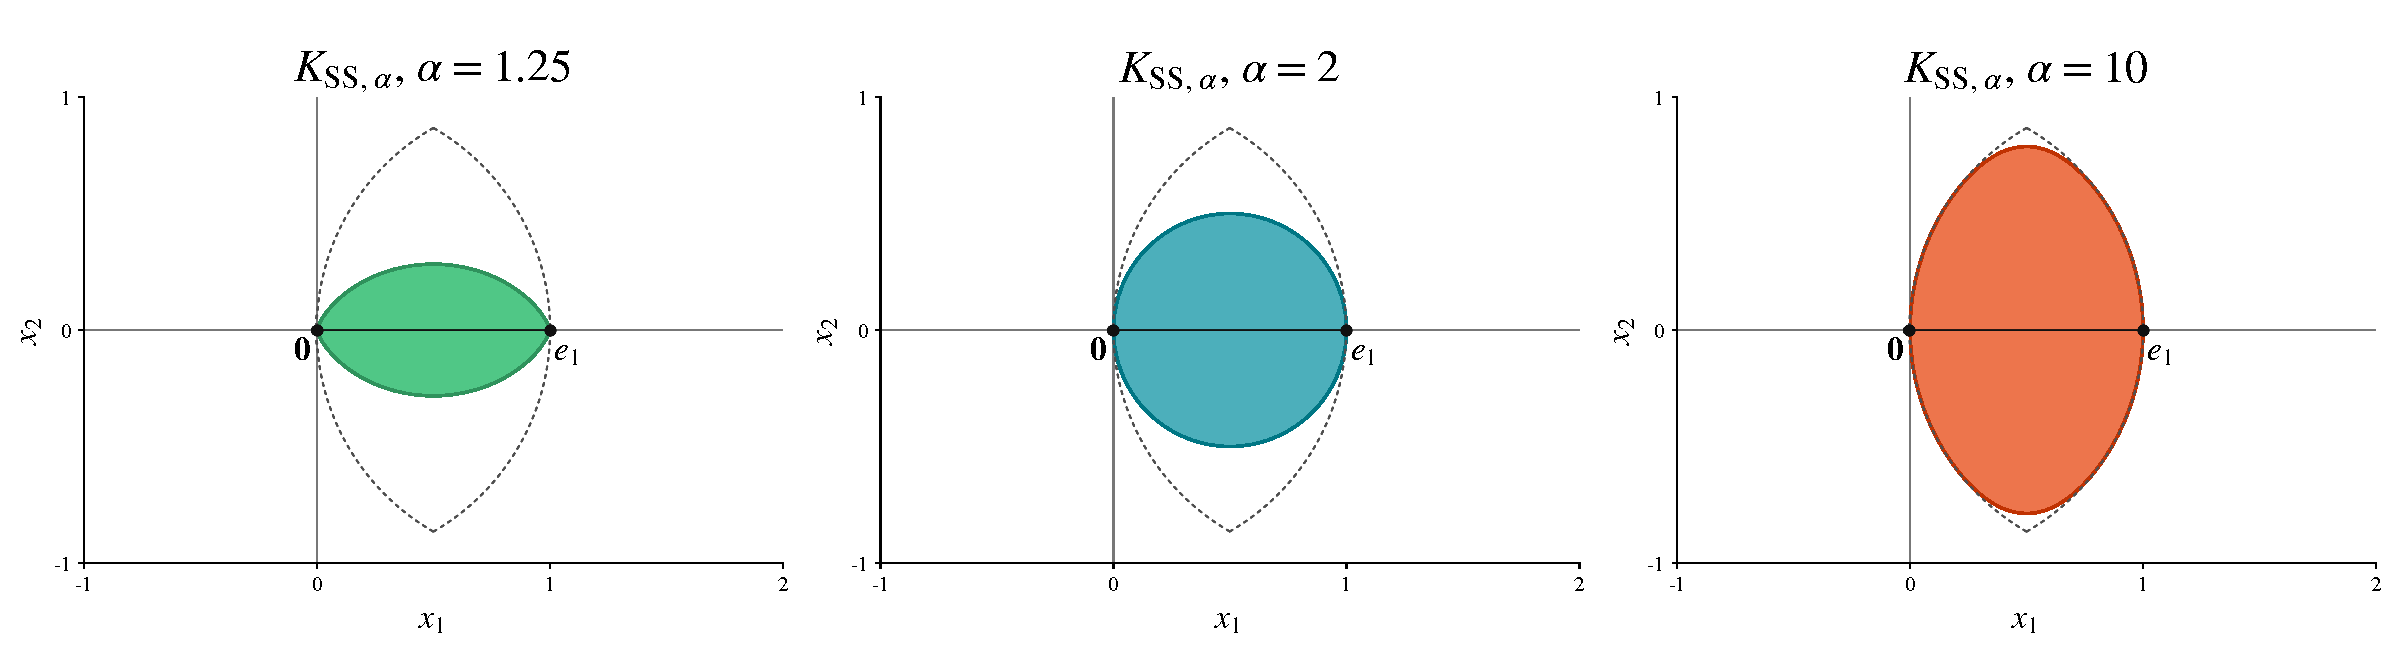
\includegraphics[width=0.98\linewidth]{stepping_stone_region_templates.pdf}
    \vspace{3pt}

    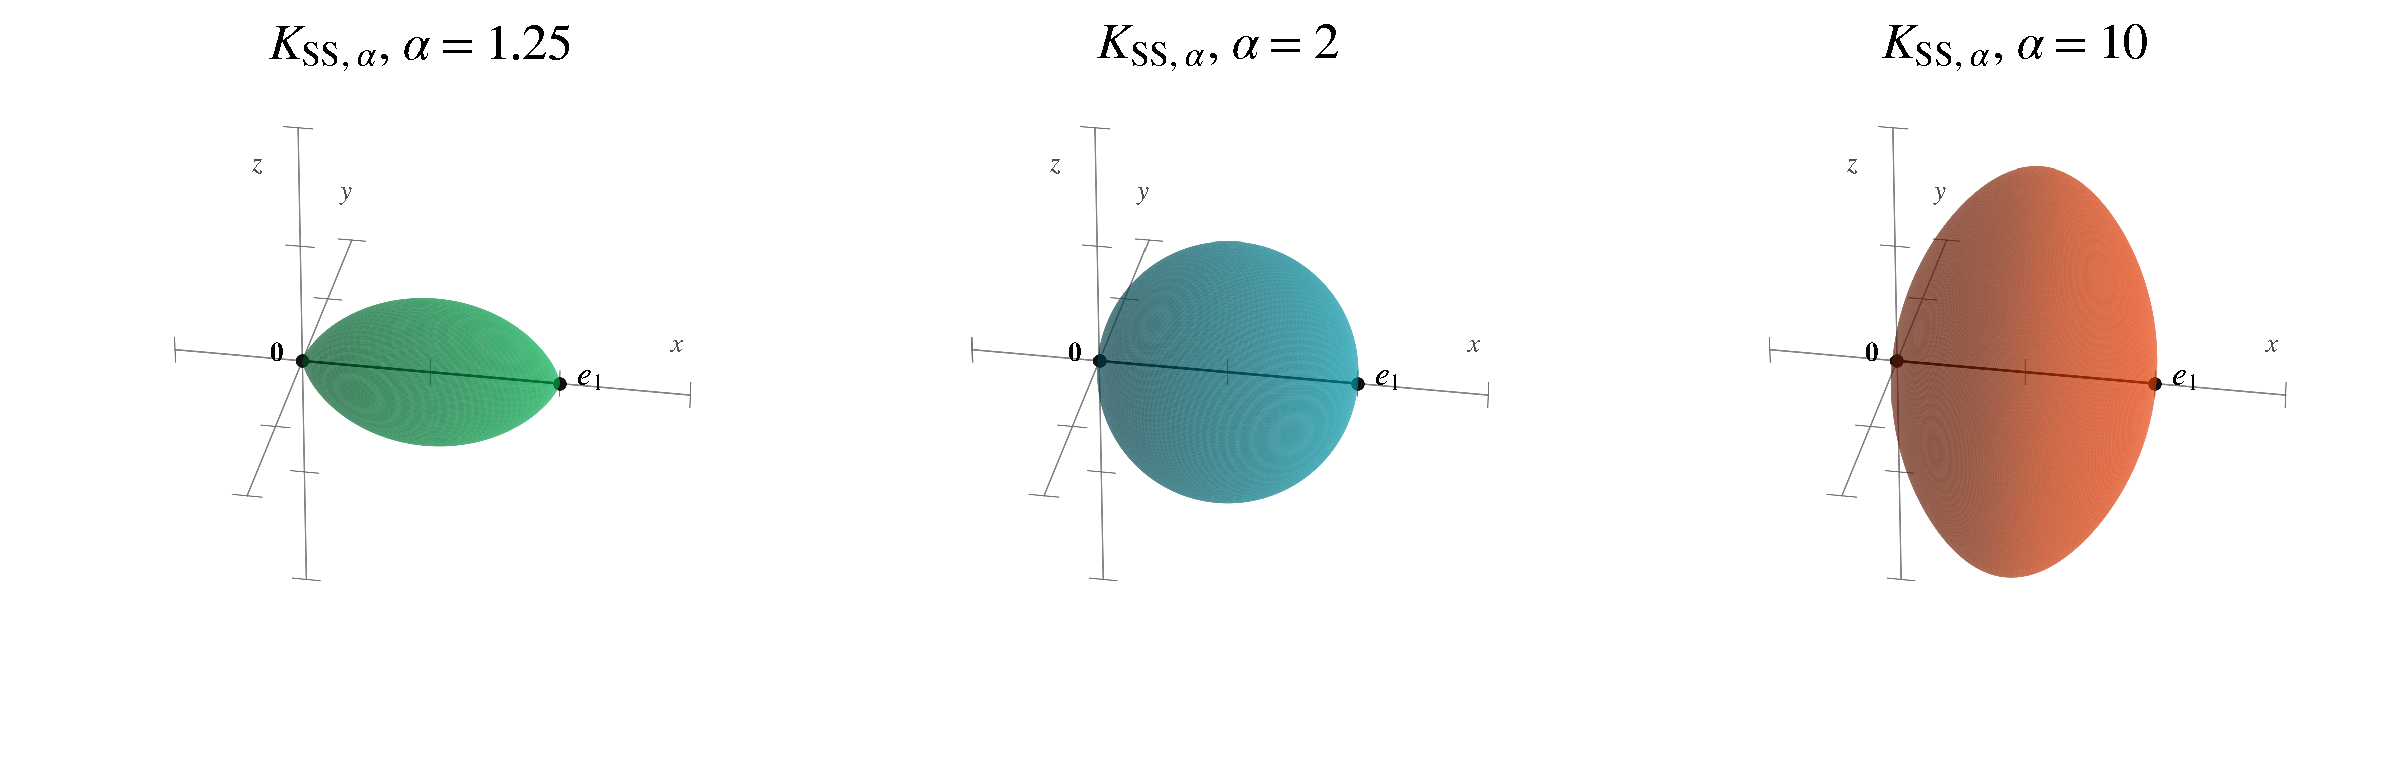
\includegraphics[width=0.98\linewidth]{stepping_stone_three_dimensional_regions.pdf}
    \vspace{-.75cm}
    \caption{Normalized stepping-stone diversion neighborhoods for
    $\alpha=1.25$, $2$, and $10$. Top: planar regions, with the limiting
    relative-neighborhood lune shown by the dashed boundary. Bottom:
    three-dimensional regions for the same parameter values. The defining
    sites are fixed at $\0$ and $e_1$.}
    \label{fig:ss-regions}
\end{figure*}
% \FloatBarrier

To complement the static views in \Cref{fig:ss-regions}, the computational
companion~\citep{espino2026computational} provides an
\href{https://heri-espino.github.io/Stepping-Stone-Volume-Constants/}
{interactive three-dimensional visualization} of the normalized diversion
neighborhood. 

\begin{proposition}[Elementary geometry]\label{prop:geometry}
For every $\alpha\geq1$, the region $S_{\mathrm{SS},\alpha}(p,q)$ is compact
and convex. It is centrally symmetric about
\begin{equation}
    m:=\frac{p+q}{2},
\end{equation}
rotationally symmetric about the line through $p$ and $q$ 
and invariant under every Euclidean isometry fixing the line through
$p$ and $q$ pointwise. If
$\alpha>1$, then $S_{\mathrm{SS},\alpha}(p,q)$ has nonempty interior and is
strictly convex.
\end{proposition}

\begin{proof}
The function
\begin{equation}
    F_{p,q,\alpha}(z)
    :=\norm{z-p}^{\alpha}+\norm{z-q}^{\alpha}
\end{equation}
is continuous and convex for $\alpha\geq1$. Hence its sublevel set
$S_{\mathrm{SS},\alpha}(p,q)$ is closed and convex. Its defining inequality
implies
\begin{equation}
    \norm{z-p}\leq\ellpq,
    \qquad
    \norm{z-q}\leq\ellpq,
\end{equation}
so the region is bounded and therefore compact.

The reflection $z\mapsto p+q-z$ exchanges the two distance terms and preserves
the region, invariant under every Euclidean isometry fixing the line through
$p$ and $q$ pointwise and therefore proving central symmetry.
Every rotation about the line through
$p$ and $q$ preserves both distances and therefore preserves the region.

For $\alpha>1$, the map $z\mapsto\norm{z-p}^{\alpha}$ is strictly convex, and
so is $F_{p,q,\alpha}$. If $z_1\neq z_2$ belong to the region and
$t\in(0,1)$, then
\begin{equation}
\begin{aligned}
F_{p,q,\alpha}\bigl(tz_1+(1-t)z_2\bigr)
&<
tF_{p,q,\alpha}(z_1)
\\
&\quad
+(1-t)F_{p,q,\alpha}(z_2)
\\
&\leq \ellpq^\alpha.
\end{aligned}
\end{equation}
Thus the open segment joining $z_1$ and $z_2$ lies in the interior. Moreover,
\begin{equation}
    F_{p,q,\alpha}(m)
    =2\left(\frac{\ellpq}{2}\right)^{\alpha}
    =2^{1-\alpha}\ellpq^{\alpha}
    <\ellpq^{\alpha},
\end{equation}
so the interior is nonempty.
\end{proof}


\section{Boundary parametrization and volume}
\label{sec:boundary-volume}

All results in this section are valid for every ambient dimension $d\geq2$;
the planar formula is recorded afterward only as a special case.

\subsection{Boundary parametrization}

We work in the normalized configuration $(p,q)=(\0,e_1)$ and write
\begin{equation}
z=(X,Z),\qquad X\in\R,\qquad Z\in\R^{d-1},
\end{equation}
with transverse radius $Y:=\norm{Z}$. The boundary is specified implicitly by
\begin{equation}
\left(X^2+Y^2\right)^{\nicefrac{\alpha}{2}}
+
\left((X-1)^2+Y^2\right)^{\nicefrac{\alpha}{2}}
=1.
\end{equation}
The following result turns this implicit equation into the boundary profile
used throughout the volume calculation.

\begin{proposition}[Boundary parametrization]
\label{prop:boundary-parametrization}
Let $\alpha>1$ and set $u_0:=2^{-\nicefrac{1}{\alpha}}$. For
$u\in[u_0,1]$, define
\begin{equation}
\rho(u):=(1-u^\alpha)^{\nicefrac{1}{\alpha}},
\qquad
X_\alpha(u):=\frac{1+u^2-\rho(u)^2}{2},
\end{equation}
and define the midpoint-centered axial coordinate and transverse radius by
\begin{align}
x_\alpha(u)
:&=X_\alpha(u)-\frac12
=\frac{
u^2-(1-u^\alpha)^{\nicefrac{2}{\alpha}}
}{2},
\label{eq:x-alpha}
\\
y_\alpha(u)
:&=\sqrt{u^2-X_\alpha(u)^2}
\notag
\\
&=\frac12\Bigl[
4u^2
-\bigl(
1+u^2-(1-u^\alpha)^{\nicefrac{2}{\alpha}}
\bigr)^2
\Bigr]^{\nicefrac12}.
\label{eq:y-alpha}
\end{align}
Then $(X_\alpha(u),y_\alpha(u))$ traces the complete boundary profile in the
half-space $X\geq \nicefrac{1}{2}$; orthogonal transformations
fixing the $e_1$-axis give the complete right
boundary of $K_{\mathrm{SS},\alpha}$. Moreover,
\begin{equation}
x_\alpha(u_0)=0,
\qquad
x_\alpha(1)=\frac12,
\end{equation}
and
\begin{equation}\label{eq:x-prime}
x_\alpha'(u)
=
u+u^{\alpha-1}(1-u^\alpha)^{\nicefrac{(2-\alpha)}{\alpha}}>0,
\qquad (u_0\leq u<1).
\end{equation}
Thus $x_\alpha$ maps $[u_0,1]$ continuously and strictly increasingly onto
$[0,\nicefrac{1}{2}]$.
\end{proposition}

\begin{proof}
Parametrize a boundary point by its distance to the first site,
$u:=\norm z$. Its distance to the second site is then $\rho(u)$ because
$u^\alpha+\rho(u)^\alpha=1$. On the right half, $u\geq\rho(u)$, which is
equivalent to $u\geq u_0$; the endpoint $u=1$ is the site $e_1$.
The two sphere equations
\begin{equation}
X^2+Y^2=u^2,
\qquad
(X-1)^2+Y^2=\rho(u)^2
\end{equation}
give $2X-1=u^2-\rho(u)^2$, and hence
\eqref{eq:x-alpha}--\eqref{eq:y-alpha}. Conversely, for every
$u\in[u_0,1]$ we have
\begin{equation}
u+\rho(u)\geq u^\alpha+\rho(u)^\alpha=1,
\qquad
|u-\rho(u)|\leq1,
\end{equation}
so the two spheres intersect and \eqref{eq:y-alpha} is real. These equations
therefore construct a boundary point, and every boundary point in the right
half has exactly one value of $u$. The endpoint identities follow by
substitution. Differentiating \eqref{eq:x-alpha} gives
\eqref{eq:x-prime}, whose two terms are positive on $[u_0,1)$. For
$\alpha>2$, the second term has an endpoint singularity at $u=1$. Since
$1-u^\alpha\sim\alpha(1-u)$ and $\nicefrac{2}{\alpha}-1>-1$, the singularity is
integrable; the integrals below are interpreted as improper integrals in that
case.
\end{proof}

\begin{figure}[pos=ht]
\centering
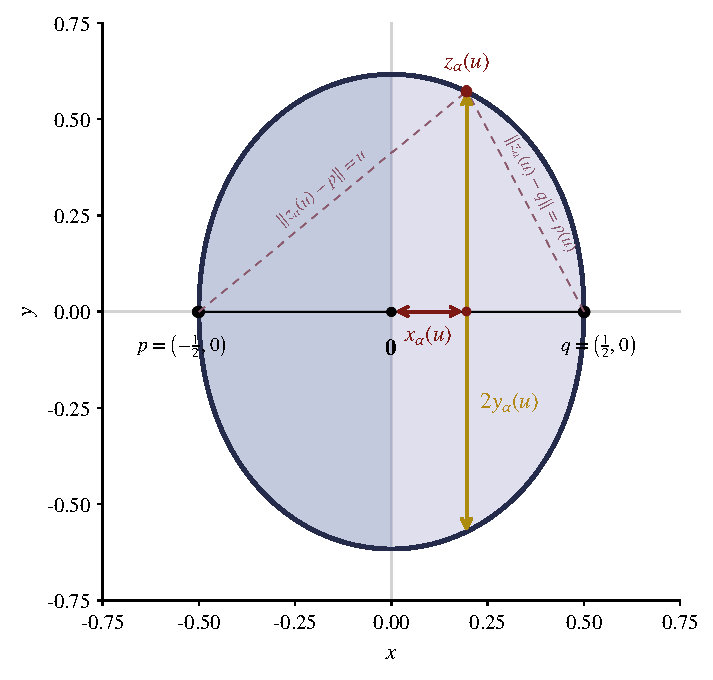
\includegraphics[width=1\linewidth]{stepping_stone_proof_midpoint.pdf}
\vspace{-.05cm}
\caption{Midpoint-centered slicing of $K_{\mathrm{SS},\alpha}$. The right
half is parametrized by $x=x_\alpha(u)$, and the transverse radius is
$y_\alpha(u)$.}
\label{fig:ss-proof-midpoint}
\end{figure}
% \FloatBarrier

\subsection{One-dimensional volume formula}

\begin{theorem}[One-dimensional volume formula]\label{thm:main}
Let $d\geq2$ and $\alpha>1$. Then
\begin{equation}\label{eq:main-integral}
 a_{d,\mathrm{SS}}(\alpha)
 =
 2\kappa_{d-1}
 \int_{2^{-\nicefrac{1}{\alpha}}}^1
 y_{\alpha}(u)^{d-1}x_{\alpha}'(u)\dd u,
\end{equation}
where $y_\alpha$ and $x_\alpha'$ are given by \eqref{eq:y-alpha} and
\eqref{eq:x-prime}. Together with \Cref{prop:factorization}, this determines
the volume for every pair of distinct sites in $\R^d$.
\end{theorem}

\begin{proof}
Every point \(z=(X,Z)\) in the normalized region satisfies
\(0\leq X\leq1\). Indeed, \eqref{eq:unit-region} implies
\begin{equation}
\norm z\leq1
\qquad\text{and}\qquad
\norm{z-e_1}\leq1,
\end{equation}
since both terms on its left-hand side are nonnegative. If \(X<0\),
then
\begin{equation}
\norm{z-e_1}\geq |1-X|=1-X>1,
\end{equation}
whereas, if \(X>1\), then
\begin{equation}
\norm z\geq |X|=X>1.
\end{equation}
Both cases contradict the preceding necessary inequalities. Hence the
normalized region is contained in the slab \(0\leq X\leq1\).

For \(x\in[0,\nicefrac{1}{2}]\), define the transverse section
\begin{equation}
\mathcal S_x
:=
\set{Z\in\R^{d-1}:(x+\nicefrac{1}{2},Z)\in K_{\mathrm{SS},\alpha}}.
\end{equation}
By \Cref{prop:geometry}, \(\mathcal S_x\) is compact, convex, and
invariant under every orthogonal transformation of \(\R^{d-1}\).
Moreover, \(0\in\mathcal S_x\), since the segment
\([\0,e_1]\) is contained in the normalized region.

Let
\begin{equation}
R(x):=\max\set{\norm Z:Z\in\mathcal S_x},
\end{equation}
where the maximum exists by compactness. If
\(Z_\ast\in\mathcal S_x\) satisfies \(\norm{Z_\ast}=R(x)\), orthogonal
invariance implies that
\begin{equation}
\set{Z\in\R^{d-1}:\norm Z=R(x)}
\subseteq\mathcal S_x.
\end{equation}
Since \(\mathcal S_x\) is convex, it contains the convex hull of this
sphere, namely the closed ball of radius \(R(x)\). Conversely, the
definition of \(R(x)\) implies that every \(Z\in\mathcal S_x\) satisfies
\(\norm Z\leq R(x)\). Hence
\begin{equation}
\mathcal S_x
=
\set{Z\in\R^{d-1}:\norm Z\leq R(x)},
\end{equation}
and therefore
\begin{equation}
\lambda_{d-1}(\mathcal S_x)
=
\kappa_{d-1}R(x)^{d-1}.
\end{equation}   

By \Cref{prop:boundary-parametrization}, the boundary of the right half is
given by $x=x_\alpha(u)$ and
$R(x_\alpha(u))=y_\alpha(u)$ for $u\in[u_0,1]$, and $x_\alpha$ is a valid
change of variables from $[u_0,1]$ onto $[0,\nicefrac{1}{2}]$.

By Cavalieri's principle,
\begin{equation}
\lambda_d(K_{\mathrm{SS},\alpha}\cap\{X\geq\nicefrac{1}{2}\})
=
\int_0^{\nicefrac{1}{2}}\kappa_{d-1}R(x)^{d-1}\dd x.
\end{equation}
Changing variables from $x$ to $u$ gives
\begin{equation}
\lambda_d(K_{\mathrm{SS},\alpha}\cap\{X\geq\nicefrac{1}{2}\})
=
\kappa_{d-1}
\int_{u_0}^{1}y_\alpha(u)^{d-1}x_\alpha'(u)\dd u.
\end{equation}
Finally, the reflection $(X,Z)\mapsto(1-X,Z)$ preserves $K_{\mathrm{SS},\alpha}$ and exchanges the two halves. The midpoint hyperplane has zero $d$-dimensional Lebesgue measure, so multiplying the last display by $2$ proves \eqref{eq:main-integral}.
\end{proof}

\begin{remark}[Planar specialization]
For $d=2$, $\kappa_{d-1}=\kappa_1=2$, and therefore
\begin{equation}
 a_{2,\mathrm{SS}}(\alpha)
 =
 4\int_{2^{-\nicefrac{1}{\alpha}}}^1
 y_{\alpha}(u)x_{\alpha}'(u)\dd u.
\end{equation}
\end{remark}


\subsection{Special and limiting cases}

The graph identity at $\alpha=2$ was established in the original planar
stepping-stone study by
\citet[Theorem~3.4]{kannangara2018stepping}. The next proposition records
the corresponding diversion regions and their normalized volumes in every
dimension, together with the degenerate case $\alpha=1$.

\begin{proposition}[Degenerate and Gabriel graph region cases]
\label{prop:special-cases}
For every $d\geq2$,
\begin{equation}\label{eq:degenerate-constant}
a_{d,\mathrm{SS}}(1)=0,
\end{equation}
whereas
\begin{equation}\label{eq:gabriel-constant}
a_{d,\mathrm{SS}}(2)=\frac{\kappa_d}{2^d}.
\end{equation}
At $\alpha=1$, the diversion neighborhood is the segment $[p,q]$; at $\alpha=2$,
it is the closed ball with diameter $pq$.
In particular, $\SSG_2(V)=\GG(V)$ for every finite or locally finite
point set $V$. At $\alpha=1$, two sites are adjacent exactly when the open segment
joining them contains no other point of $V$; consequently,
$\SSG_1(V)$ is complete whenever no three points of $V$ are collinear.
\end{proposition}

\begin{proof}
At $\alpha=1$, the triangle inequality shows that
\begin{equation}
\norm{z-p}+\norm{z-q}\leq\ellpq
\end{equation}
holds precisely on the segment joining $p$ and $q$, which has zero
$d$-dimensional measure. At $\alpha=2$, let $m=\nicefrac{(p+q)}{2}$. The parallelogram
identity gives
\begin{equation}
\norm{z-p}^2+\norm{z-q}^2
=
2\norm{z-m}^2+2\left(\frac{\ellpq}{2}\right)^2.
\end{equation}
Thus the region is the ball centered at $m$ with radius $\nicefrac{\ellpq}{2}$, and its
normalized volume is $\nicefrac{\kappa_d}{2^d}$.
The graph identity follows from the closed-ball convention in the
definition of $\GG(V)$. The characterization at $\alpha=1$ follows
by deleting the two defining sites from the segment $[p,q]$.
\end{proof}


The convergence of the planar graph to the relative-neighborhood graph was
identified by \citet[Theorem~3.5]{kannangara2018stepping}. The following
result strengthens that statement by identifying the increasing union of the
diversion regions and the limiting volume in arbitrary dimension.


\begin{proposition}[Convergence to the relative-neighborhood lune]
\label{prop:rng-limit}
Define the normalized relative-neighborhood volume constant by
\begin{equation}
    a_{d,\mathrm{RNG}}
    :=
    \lambda_d\bigl(L_{\mathrm{op}}(\0,e_1)\bigr)
    =
    \lambda_d\bigl(L_{\mathrm{cl}}(\0,e_1)\bigr).
\end{equation}
As $\alpha\to\infty$, the diversion neighborhoods converge from within to
the open relative-neighborhood lune in the precise sense that
\begin{equation}\label{eq:open-lune-limit}
\bigcup_{1<\alpha<\infty}
\left(S_{\mathrm{SS},\alpha}(p,q)\setminus\{p,q\}\right)
=
L_{\mathrm{op}}(p,q).
\end{equation}
Moreover,
\begin{equation}\label{eq:rng-constant}
    \lim_{\alpha\to\infty}
    a_{d,\mathrm{SS}}(\alpha)
    =
    a_{d,\mathrm{RNG}}
    =
    \kappa_d
    I_{\nicefrac{3}{4}}\left(\frac{d+1}{2},\frac12\right).
\end{equation}
where $I_{\nicefrac{3}{4}}$ is the regularized incomplete beta function.

\end{proposition}
\begin{proof}
For $z\notin\{p,q\}$, the defining inequality implies the strict bounds
\begin{equation}
\|z-p\|< \ell_{p,q},
\qquad
\|z-q\|< \ell_{p,q}.
\end{equation}
Thus every finite-parameter diversion neighborhood, after removing its defining
sites, is contained in $L_{\mathrm{op}}(p,q)$.

Conversely, let \(z\in L_{\mathrm{op}}(p,q)\). Then
\begin{equation}
0\leq \frac{\|z-p\|}{\ell_{p,q}}<1,
\qquad
0\leq \frac{\|z-q\|}{\ell_{p,q}}<1,
\end{equation}
and consequently
\begin{equation}
\left(\frac{\|z-p\|}{\ell_{p,q}}\right)^\alpha
+
\left(\frac{\|z-q\|}{\ell_{p,q}}\right)^\alpha
\longrightarrow 0
\qquad\text{as }\alpha\to\infty.
\end{equation}
Hence, for all sufficiently large \(\alpha\),
\begin{equation}
\|z-p\|^\alpha+\|z-q\|^\alpha
\leq \ell_{p,q}^\alpha,
\end{equation}
so \(z\in S_{\mathrm{SS},\alpha}(p,q)\).

% This proves \eqref{eq:open-lune-limit}. The same eventual-membership argument
% shows that
% \begin{equation}
% \mathbf{1}_{S_{\mathrm{SS},\alpha}(p,q)\setminus\{p,q\}}(z)
% \longrightarrow
% \mathbf{1}_{L_{\mathrm{op}}(p,q)}(z)
% \end{equation}
% for every \(z\in\R^d\). Since deleting the two defining sites does not change
% Lebesgue measure and all these sets lie in the bounded closed lune, dominated
% convergence yields
This proves \eqref{eq:open-lune-limit}. Since membership is eventually
constant at every point, the neighborhoods lie in the bounded closed lune,
and deleting their two defining sites does not change Lebesgue measure,
dominated convergence yields
\begin{equation}
    \lim_{\alpha\to\infty}
    \lambda_d\bigl(S_{\mathrm{SS},\alpha}(p,q)\bigr)
    =
    \lambda_d\bigl(L_{\mathrm{cl}}(p,q)\bigr).
\end{equation}

The volume of the unit relative-neighborhood lune in arbitrary dimension was
previously represented as a radial integral by
\citet[Sec.~5, p.~59]{devroye1988expected}. Equivalently, in normalized
coordinates, the midpoint hyperplane partitions
$L_{\mathrm{cl}}(\0,e_1)$ into two congruent unit-ball caps of height $\nicefrac{1}{2}$.
The standard hyperspherical-cap formula of \citet{li2011concise} gives one cap
volume
\begin{equation}
\frac{\kappa_d}{2}
I_{\nicefrac{3}{4}}\left(\frac{d+1}{2},\frac12\right).
\end{equation}
Doubling proves \eqref{eq:rng-constant}. For example, in dimension three the benchmarks corresponding to the Gabriel graph and relative-neighborhood-graph benchmarks are $a_{3,\mathrm{SS}}(2)=\nicefrac{\pi}{6}$ and
$a_{3,\mathrm{RNG}}=\nicefrac{5\pi}{12}$, respectively.
\end{proof}


\section{Monotonicity and graph consequences}
\label{sec:monotonicity-graphs}

% The region, volume, and graph results in this section hold in arbitrary
% dimension. The Delaunay containment in the final remark is also
% dimension independent; only the linear candidate bound and the cited
% stepping-stone algorithm are specific to the plane.

% The strict region and volume results, the graph inclusion chains,
% connectivity, and finite-parameter stabilization established in this section
% hold in every ambient dimension. The containment in the Delaunay and Gabriel graphs also
% remain valid in arbitrary dimension. \tb{The linear planar candidate bound,
% however, is dimension-specific, and the corresponding candidate graphs may
% already have quadratic size in dimension three.} % No me queda claro en esta frase sobre que es la "candidate bound", ni sobre que se aplica el "quadratic size". Creo que podría mejorarse esta oración.

The strict region and volume results, the graph inclusion chains,
connectivity, and finite-parameter stabilization established in this section
hold in every ambient dimension. 
The containment in the Delaunay and Gabriel graphs also
remain valid in arbitrary dimension.

The linear bound on the number of Delaunay edges used as an initial
candidate set is specific to the plane. In dimension three, both Delaunay
and Gabriel graphs may have quadratic size, so neither containment yields a
subquadratic worst-case set of edges to be tested.


\subsection{Strict region and volume monotonicity}

The monotone decrease of the planar stepping-stone graph with the
configuration parameter is due to
\citet[Theorem~3.3]{kannangara2018stepping}. The next theorem proves the
strict geometric refinement needed here: strict inclusion of the diversion
regions, positive measure of their difference, and strict monotonicity of the
normalized volume in every dimension.


\begin{theorem}[Strict monotonicity]\label{thm:monotonicity}
For every $1\leq\alpha_1<\alpha_2$ and every distinct $p,q\in\R^d$,
\begin{equation}
S_{\mathrm{SS},\alpha_1}(p,q)
\subsetneq
S_{\mathrm{SS},\alpha_2}(p,q),
\end{equation}
and the set difference has positive $d$-dimensional measure. Consequently,
\begin{equation}
 a_{d,\mathrm{SS}}(\alpha_1)<a_{d,\mathrm{SS}}(\alpha_2).
\end{equation}
\end{theorem}

\begin{proof}
For $a,b\geq0$, the map
\begin{equation}
    r\longmapsto \left(a^r+b^r\right)^{\nicefrac{1}{r}},
    \qquad r>0,
\end{equation}
is nonincreasing. If $z\in S_{\mathrm{SS},\alpha_1}(p,q)$, then
\begin{equation}
\bigl(\norm{z-p}^{\alpha_1}+\norm{z-q}^{\alpha_1}\bigr)^{\nicefrac{1}{\alpha_1}}
\leq \ellpq.
\end{equation}
The monotonicity of this map gives
\begin{equation}
\begin{aligned}
\bigl(r^{\alpha_2}+s^{\alpha_2}\bigr)^{
\nicefrac{1}{\alpha_2}}
&\leq
\bigl(r^{\alpha_1}+s^{\alpha_1}\bigr)^{
\nicefrac{1}{\alpha_1}}
\\
&\leq \ellpq,
\end{aligned}
\end{equation}
so $z\in S_{\mathrm{SS},\alpha_2}(p,q)$. Taking Lebesgue
measure and using \eqref{eq:volume-factorization} gives the volume
monotonicity.

The monotonicity of this map gives
\begin{equation}
\begin{aligned}
\bigl(r^{\alpha_2}+s^{\alpha_2}\bigr)^{
\nicefrac{1}{\alpha_2}}
&\leq
\bigl(r^{\alpha_1}+s^{\alpha_1}\bigr)^{
\nicefrac{1}{\alpha_1}}
\\
&\leq \ellpq,
\end{aligned}
\end{equation}
so $z\in S_{\mathrm{SS},\alpha_2}(p,q)$. Taking Lebesgue
measure and using \eqref{eq:volume-factorization} gives the volume
monotonicity.

To prove strictness, let $m=\nicefrac{(p+q)}{2}$ and choose a unit vector $v$
perpendicular to $q-p$. On the midpoint hyperplane, a point $z=m+tv$ belongs
to $S_{\mathrm{SS},\alpha}(p,q)$ precisely when
\begin{equation}
    |t|\leq r_{\alpha},
    \qquad
    r_{\alpha}
    :=
    \ellpq\sqrt{2^{-\nicefrac{2}{\alpha}}-\frac14}.
\end{equation}
The function $\alpha\mapsto2^{-\nicefrac{2}{\alpha}}$ is strictly increasing, so
$r_{\alpha_1}<r_{\alpha_2}$. Choose $t$ strictly between these two radii.
Then $m+tv$ lies in the interior of the larger region and outside the closed
smaller region. A neighborhood of this point is therefore contained in the
set difference, which has positive $d$-dimensional measure. The strict
inequality for the normalized volumes follows from
\eqref{eq:volume-factorization}.
\end{proof}


\begin{corollary}[Continuous parameter calibration]
\label{cor:continuous-calibration}
For every $d\geq2$, the map
$\alpha\mapsto a_{d,\mathrm{SS}}(\alpha)$ is continuous and strictly
increasing on $[1,\infty)$, with image
$[0,a_{d,\mathrm{RNG}})$. Consequently, every target volume
$c\in(0,a_{d,\mathrm{RNG}})$ determines a unique finite parameter
$\alpha>1$.
\end{corollary}

\begin{proof}
Let $\alpha_n\to\alpha\geq1$. Away from the boundary of
$K_{\mathrm{SS},\alpha}$, continuity of the defining inequality implies
eventual agreement of membership in $K_{\mathrm{SS},\alpha_n}$ and
$K_{\mathrm{SS},\alpha}$. This boundary has Lebesgue measure zero: for
$\alpha>1$ it is the boundary of a convex body, while for $\alpha=1$ the
entire region is a line segment. All these regions are contained in the
bounded closed relative-neighborhood lune, so dominated convergence proves
continuity of their volumes. The image and uniqueness now follow from
\Cref{prop:special-cases,prop:rng-limit,thm:monotonicity}.
\end{proof}

\begin{corollary}[Bounds and Gabriel graph region comparison]\label{cor:bounds}
For every $d\geq2$, the following holds:
\begin{equation}
\begin{cases}
a_{d,\mathrm{SS}}(\alpha)=0, & \alpha=1,\\[1mm]
0<a_{d,\mathrm{SS}}(\alpha)<\kappa_d/2^d, & 1<\alpha<2,\\[1mm]
a_{d,\mathrm{SS}}(\alpha)=\kappa_d/2^d, & \alpha=2,\\[1mm]
\kappa_d/2^d<a_{d,\mathrm{SS}}(\alpha)<a_{d,\mathrm{RNG}},
    & 2<\alpha<\infty.
\end{cases}
\end{equation}
Moreover, for every distinct $p,q\in\R^d$,
\begin{equation}
S_{\mathrm{SS},\alpha}(p,q)\subsetneq \GG_{\mathrm{cl}}(p,q)
\quad (1\leq\alpha<2),
\end{equation}
whereas $\GG_{\mathrm{cl}}(p,q)\subsetneq S_{\mathrm{SS},\alpha}(p,q)$ for every
$2<\alpha<\infty$.
\end{corollary}

\begin{proof}
Combine \Cref{prop:special-cases,prop:rng-limit,thm:monotonicity}. The strict
upper bound by $a_{d,\mathrm{RNG}}$ at every finite parameter follows because
a strictly increasing function cannot attain its limiting value at a finite
argument.
\end{proof}

\subsection{Monotonicity and graph inclusions}
\label{sec:inclusions}

For $i\in\{1,2\}$, let $S_i(p,q)$ be a region assigned to each pair of
distinct sites, and let $G_i(V)=(V,E_i(V))$ join $p$ and $q$ precisely when
$S_i(p,q)$ contains no point of $V\setminus\{p,q\}$. Directly from this
definition, whenever the region inclusion below holds for every distinct pair,
so does the edge inclusion:
\begin{equation}
\begin{aligned}
S_1(p,q)\setminus\{p,q\}
&\subseteq
S_2(p,q)\setminus\{p,q\}
\\
&\Longrightarrow
E_2(V)\subseteq E_1(V).
\end{aligned}
\end{equation}
Indeed, if the intersection of $S_2(p,q)$ with
$V\setminus\{p,q\}$ is empty, then the corresponding intersection with
$S_1(p,q)$ is also empty.

Let $\MST(V)$ denote a Euclidean minimum spanning tree of a
nonempty finite point set $V$, and let $\Del(V)$ denote its Delaunay graph
\citep{mitchell2018}. With the closed Gabriel-ball and open
relative-neighborhood lune conventions adopted above, the standard
inclusions are
\begin{equation}
    \MST(V)\subseteq\RNG(V)\subseteq\GG(V)\subseteq\Del(V).
\end{equation}
The hierarchy is reviewed by \citet{jaromczyk1992relative}; the
closed-ball Gabriel convention and the corresponding inclusion in the Delaunay graph are explicit in
\citet{matula1980properties} and
\citet{cardinal2009empty}. 
In particular, an empty closed ball with diameter $pq$ 
certifies that $pq$ is a Delaunay edge, including in configurations 
with cospherical sites.


In the planar setting, the parameter endpoint cases corresponding to the Gabriel and relative-neighborhood graphs, and the containment in the Delaunay graph for parameters
at least two were established by
\citet[Theorems~3.3--3.5 and~3.11]{kannangara2018stepping}. The next
proposition gives a region-based derivation that makes the open--closed
conventions explicit and extends the resulting inclusion chains to every
ambient dimension.

\begin{proposition}[Monotonicity and classical proximity-graph inclusions]
\label{prop:inclusions}
If $1\leq\alpha_1<\alpha_2$, then
\begin{equation}\label{eq:ss-edge-monotonicity}
    E_{\alpha_2}(V)\subseteq E_{\alpha_1}(V).
\end{equation}
Thus $\{\SSG_\alpha(V):\alpha\geq1\}$ is a monotonically decreasing family
of graphs under edge inclusion, although the inclusion need not be strict for
a fixed point set.
Furthermore, for every nonempty finite $V\subset\R^d$ and every finite
$\alpha\geq1$,
\begin{equation}
    \MST(V)\subseteq\RNG(V)\subseteq\SSG_\alpha(V).
\end{equation}
If $1\leq\alpha\leq2$, then
\begin{equation}
    \MST(V)\subseteq\RNG(V)\subseteq\GG(V)
    \subseteq\SSG_\alpha(V).
\end{equation}
If $\alpha\geq2$, then
\begin{equation}\label{eq:tail-chain}
\begin{aligned}
\MST(V)\subseteq\RNG(V)
&\subseteq\SSG_\alpha(V)
\\
&\subseteq\GG(V)\subseteq\Del(V).
\end{aligned}
\end{equation}
\end{proposition}

\begin{proof}
The first edge inclusion follows directly from \Cref{thm:monotonicity} and
the preceding implication; it is the region-inclusion formulation of the
nestedness proved for the original $d$-spectrum by
\citet{kannangara2018stepping,kannangara2019stepping}.

For $z\notin\{p,q\}$, the inequality defining
$S_{\mathrm{SS},\alpha}(p,q)$ implies
\begin{equation}
    \norm{z-p}<\ellpq,
    \qquad
    \norm{z-q}<\ellpq.
\end{equation}
Thus
$S_{\mathrm{SS},\alpha}(p,q)\setminus\{p,q\}
\subset L_{\mathrm{op}}(p,q)$,
and the same implication gives $\RNG(V)\subseteq\SSG_\alpha(V)$. The remaining
stepping-stone inclusions follow from
\Cref{prop:special-cases,thm:monotonicity}; the other inclusions are
classical.
\end{proof}

\begin{corollary}[Connectivity in arbitrary dimension]
\label{cor:graph-consequence}
For every nonempty finite \(V\subset\R^d\) and every finite
\(\alpha\geq1\),
the graph \(\SSG_\alpha(V)\) is connected.
\end{corollary}

\begin{proof}
Connectivity follows from
\begin{equation}
\MST(V)\subseteq\RNG_{\mathrm{op}}(V)
\subseteq\SSG_\alpha(V).
\end{equation}
Therefore, \(\SSG_\alpha(V)\) contains a connected spanning subgraph and
is itself connected.
\end{proof}

\begin{corollary}[Finite-parameter stabilization]
\label{cor:finite-stabilization}
For every finite $V\subset\R^d$, there exists a finite parameter
$\alpha_\ast(V)\geq1$ such that
\begin{equation}
    \SSG_\alpha(V)=\RNG_{\mathrm{op}}(V)
    \qquad\text{for all }\alpha\geq\alpha_\ast(V).
\end{equation}
\end{corollary}

\begin{proof}
For every pair $p,q\in V$ that is not an edge of
$\RNG_{\mathrm{op}}(V)$, choose a point
$z\in L_{\mathrm{op}}(p,q)\cap(V\setminus\{p,q\})$.
By \Cref{prop:rng-limit}, that point belongs to
$S_{\mathrm{SS},\alpha}(p,q)$ for every sufficiently large $\alpha$.
There are only finitely many such pairs, so their individual thresholds
have a finite maximum $\alpha_\ast(V)$; if there are no such pairs, take
$\alpha_\ast(V)=1$. Beyond this threshold, no non-relative-neighborhood
edge remains, while \Cref{prop:inclusions} preserves every
relative-neighborhood edge.
\end{proof}

\begin{remark}[Dependence and provenance of the stabilization threshold]
\label{rem:stabilization-threshold}
In the planar case, finite stabilization is already implicit in the
finite deletion thresholds of the \(d\)-spectrum introduced by
\citet[Def.~3.12]{kannangara2018stepping}; the preceding argument extends
the observation to every fixed ambient dimension. The threshold cannot be
chosen uniformly over finite point sets. 

To see that the stabilization threshold cannot be chosen uniformly, let
$p=(0,0)$, $q=(1,0)$, and $z=(1/2,h)$, where
$0<h<\sqrt{3}/2$. Setting $r_h=\sqrt{1/4+h^2}<1$, the point $z$ enters
$S_{\mathrm{SS},\alpha}(p,q)$ precisely when
$2r_h^\alpha\leq1$, or equivalently when
\begin{equation}
\alpha\geq\frac{\log 2}{-\log r_h}.
\end{equation}
This threshold tends to infinity as $h\uparrow\sqrt{3}/2$.
\end{remark}

\begin{remark}[Planar Delaunay starting graph]
For \(V\subset\R^2\) and \(\alpha\geq2\),
\(\SSG_\alpha(V)\) is a subgraph of the Gabriel graph and hence of the
Delaunay graph. Therefore, if \(V\) is in general position and
\(n=|V|\geq3\), the defining empty-region condition need only be tested for
at most \(3n-6\) Delaunay edges, rather than for all \(\binom{n}{2}\)
pairs. Testing each candidate against the remaining \(n-2\) sites still gives
a naive \(O(n^2)\) procedure.
In their planar \(d\)-spectrum algorithm,
\citet{kannangara2018stepping,kannangara2019stepping} use the Delaunay
triangulation as the starting graph.
Although the Delaunay containment remains valid in higher dimensions,
it does not yield a subquadratic worst-case candidate set, since Delaunay
graphs can already have \(\Theta(n^2)\) edges in \(\R^3\)
\citep{agarwal1992relative}. The obstruction is not removed merely by 
restricting the initial candidate
set to Gabriel graph edges, since Gabriel graphs themselves can have
$\Theta(n^2)$ edges in $\R^3$
\citep[Lemma~5.1]{chazelle1994selecting}. Hence the candidate-edge
characterization is not, by itself, a subquadratic construction
algorithm in higher dimensions.
\end{remark}

\section{Probabilistic consequences}
\label{sec:probabilistic-consequences}

The normalized volume is also the parameter that enters the expected-size
theory of regular empty-region graphs. The first part of this section records
the arbitrary-dimensional consequences of Devroye's theorem. The second part
is an explicitly planar specialization of the graph-edge-length approximation
of \citet{watanabe2008evaluating}.
The verification below uses compactness, midpoint symmetry, and similarity
equivariance from \Cref{sec:geometry}; convexity itself is not a hypothesis in
Devroye's definition.

\subsection{Expected size in arbitrary dimension}

\begin{proposition}[Regularity in the sense of Devroye]
\label{prop:devroye-regularity}
For every fixed $\alpha>1$, the stepping-stone construction defines a regular
set in the sense of \citet{devroye1988expected}, with normalized volume
$a_{d,\mathrm{SS}}(\alpha)$.
\end{proposition}

\begin{proof}
In Devroye's terminology, take the bounded target set
\begin{equation}
\begin{split}
T_\alpha
&:=
\bigl\{(u,v)\in\R\times[0,\infty):
\\
&\qquad
(u^2+v^2)^{\nicefrac{\alpha}{2}}
+\bigl((1-u)^2+v^2\bigr)^{\nicefrac{\alpha}{2}}
\leq 1
\bigr\}.
\end{split}
\end{equation}
By \Cref{prop:geometry}, it is bounded and symmetric about $u=1/2$.
Given distinct $p,q\in\R^d$, the translation, rotation, and rescaling in
\Cref{prop:factorization} reduce membership of any point $z\in\R^d$ in
$S_{\mathrm{SS},\alpha}(p,q)$ to membership of the pair formed by its axial
coordinate and its distance from that axis in
$T_\alpha$. Allowing every transverse vector with prescribed radius
$v$ produces $K_{\mathrm{SS},\alpha}$, whose volume is
$a_{d,\mathrm{SS}}(\alpha)$. This volume is strictly positive for
$\alpha>1$ because \Cref{prop:geometry} gives nonempty interior. These
are precisely the boundedness, symmetry, and similarity requirements in
Devroye's definition of a regular set.
\end{proof}

\begin{corollary}[Expected degree and number of edges]
\label{cor:devroye-degree}
Fix \(d\geq2\) and \(\alpha>1\).
Let $X_1,\ldots,X_n$ be independent points with a common density
$f$ with respect to \(d\)-dimensional Lebesgue measure on
\(\R^d\),
and let $N_n(X_1)$ denote the number of stepping-stone neighbors of $X_1$
at parameter \(\alpha\). Then, for
$f(x)\,\mathrm{d}x$-almost every $x$,
\begin{equation}\label{eq:devroye-degree}
    \lim_{n\to\infty}
    \E\!\left[N_n(X_1)\mid X_1=x\right]
    =
    \frac{\kappa_d}{a_{d,\mathrm{SS}}(\alpha)}.
\end{equation}
If $M_n$ denotes the total number of undirected edges, then
\begin{equation}\label{eq:devroye-edge-lower-bound}
    \liminf_{n\to\infty}\frac{\E[M_n]}{n}
    \geq
    \frac{\kappa_d}{2a_{d,\mathrm{SS}}(\alpha)}.
\end{equation}
\end{corollary}

\begin{proof}
By \Cref{prop:devroye-regularity}, the volume in
Devroye's regular-set theorem is $a_{d,\mathrm{SS}}(\alpha)$, while the
volume denoted there by $V_d$ is $\kappa_d$. Substitution in the conditional
degree conclusion of that theorem gives \eqref{eq:devroye-degree}. Its
edge-count conclusion gives \eqref{eq:devroye-edge-lower-bound}; the factor
$\nicefrac{1}{2}$ appears because the sum of the vertex degrees counts every undirected
edge twice.
\end{proof}

\subsection{Planar Poisson specialization}

We now specialize to $d=2$ and use the homogeneous Poisson model of
\citet{watanabe2008evaluating}, with point intensity $\rho>0$. For brevity set
\begin{equation}
    a:=a_{2,\mathrm{SS}}(\alpha),
    \qquad \alpha>1.
\end{equation}

\begin{proposition}[Planar edge-length approximation]
\label{prop:poisson-edge-density}
Within Watanabe's approximation, let \(L\) denote the
modeled edge length for the planar stepping-stone graph generated by a
homogeneous Poisson process of intensity \(\rho\). Its distribution function
is
\begin{equation}\label{eq:watanabe-cdf}
    F_L(r)=1-\exp\{-\rho a r^2\},
    \qquad r\geq0,
\end{equation}
and its density is
\begin{equation}\label{eq:watanabe-density}
    f_L(r)
    =
    2\rho a r\exp\{-\rho a r^2\},
    \qquad r>0.
\end{equation}
Consequently
\begin{equation}\label{eq:watanabe-moments}
    \E[L]=\frac{\sqrt{\pi}}{2\sqrt{\rho a}},
    \qquad
    \operatorname{Var}(L)=\frac{4-\pi}{4\rho a}.
\end{equation}
\end{proposition}

\begin{proof}
For a pair of sites at distance $r$, the area factorization
\eqref{eq:volume-factorization} gives the area of the diversion neighborhood
\begin{equation}
    A(r)=a r^2.
\end{equation}
The Poisson probability that this region contains no point is
\begin{equation}
    \Pp\{0\text{ points in }A(r)\}\\
    =\exp\{-\rho A(r)\}
    =\exp\{-\rho a r^2\}.
\end{equation}
Within Watanabe's approximation, the probability that the restricted search
has found at least one point by distance $r$ is the complement of this void
probability; this gives \eqref{eq:watanabe-cdf}. Differentiation with respect to $r$ gives
\eqref{eq:watanabe-density}. 

For completeness, the same gamma-integral calculation gives
\begin{equation}
    \E[L]
    =2\rho a\int_0^\infty r^2e^{-\rho ar^2}\dd r
    =\frac{\Gamma(\nicefrac{3}{2})}{\sqrt{\rho a}}
    =\frac{\sqrt\pi}{2\sqrt{\rho a}}.
\end{equation}
Moreover,
\begin{equation}
    \E[L^2]
    =2\rho a\int_0^\infty r^3e^{-\rho ar^2}\dd r
    =\frac{1}{\rho a},
\end{equation}
so subtracting $\E[L]^2$ yields the variance in
\eqref{eq:watanabe-moments}. At $\alpha=2$,
\begin{equation}
a_{2,\mathrm{SS}}(2)=\nicefrac{\pi}{4},
\end{equation} 
and the formula recovers Watanabe's formula for
the Gabriel graph. As $\alpha\to\infty$,
\begin{equation}
    a_{2,\mathrm{SS}}(\alpha)
    \longrightarrow \frac{2\pi}{3}-\frac{\sqrt3}{2},
\end{equation}
which recovers his approximation for the relative-neighborhood graph.
\end{proof}

\section{Numerical evaluation and validation}
\label{sec:numerical}

\subsection{Stable quadrature}

The formula in \Cref{thm:main} is suitable for numerical evaluation, although
its original form is not always the most stable one. For $\alpha>2$,
the derivative in \eqref{eq:x-prime} diverges as $u\to1$, but the transverse
radius simultaneously tends to zero. A direct endpoint expansion gives that
\begin{equation}
    y_\alpha(u)^{d-1}x_\alpha'(u)
    \text{ is of order }
     (1-u)^{\nicefrac{(d+1)}{\alpha-1}}.
\end{equation}
Therefore, the complete integrand is unbounded only when
$\alpha>d+1$, and it remains integrable for every finite $\alpha>1$.
Nevertheless, adaptive quadrature may lose accuracy near the endpoint,
which motivates the following reparametrization.

\begin{proposition}[Stable quadrature]\label{prop:stable-quadrature}
For $\alpha>1$, define
\begin{equation}
u(t):=(1-t^\alpha)^{\nicefrac{1}{\alpha}},
\end{equation}
and
\begin{equation}
\begin{aligned}
\widetilde y_\alpha(t)
&:=\frac12\Bigl[
\bigl(u(t)+t-1\bigr)
\bigl(u(t)+t+1\bigr)
\\[-0.2em]
&\qquad{}\times
\bigl(1+u(t)-t\bigr)
\bigl(1-u(t)+t\bigr)
\Bigr]^{\nicefrac12}.
\end{aligned}
\end{equation}
Then
\begin{equation}\label{eq:stable-ss-integral}
\begin{split}
a_{d,\mathrm{SS}}(\alpha)
&=
2\kappa_{d-1}
\int_0^{2^{-\nicefrac{1}{\alpha}}}
\\[-0.2em]
&\qquad
\widetilde y_\alpha(t)^{d-1}
\left(
t+u(t)^{2-\alpha}t^{\alpha-1}
\right)
\dd t.
\end{split}
\end{equation}
and the integrand has no endpoint singularity.
\end{proposition}

\begin{proof}
Parametrize the right boundary by the distance to the second site,
\begin{equation}
t=(1-u^\alpha)^{\nicefrac{1}{\alpha}},
\qquad
u=(1-t^\alpha)^{\nicefrac{1}{\alpha}}.
\end{equation}
Then $0\leq t\leq2^{-\nicefrac{1}{\alpha}}$ and
$x=\nicefrac{(u^2-t^2)}{2}$. Since
$u'(t)=-u(t)^{1-\alpha}t^{\alpha-1}$,
\begin{equation}
\frac{\dd x}{\dd t}
=-
\left(t+u^{2-\alpha}t^{\alpha-1}\right).
\end{equation}
The coordinate $x(t)$ decreases from $\nicefrac{1}{2}$ to $0$, so the slicing formula
uses the positive element
$-\dd x=|\nicefrac{\dd x}{\dd t}|\dd t$. Substitution in \eqref{eq:main-integral}
gives \eqref{eq:stable-ss-integral}.The factorized expression for \(\widetilde y_\alpha(t)\) follows from
\begin{equation}
\begin{aligned}
4u^2-(1+u^2-t^2)^2
&=
(u+t-1)(u+t+1)
\\
&\qquad{}\cdot
(1+u-t)(1-u+t),
\end{aligned}
\end{equation}
after setting \(u=u(t)\). Finally, as \(t\to0\), we have
\(u(t)\to1\),
\(
u(t)^{2-\alpha}t^{\alpha-1}\to0
\)
because \(\alpha>1\), and
\(\widetilde y_\alpha(t)\to0\). Therefore, the integrand extends
continuously to the left endpoint and has no endpoint singularity.
\end{proof}

Evaluating the transverse radius in this factored form reduces the
cancellation caused by subtracting two nearly equal squared quantities;
all four factors are nonnegative on the integration interval.
The degenerate case is evaluated separately using
$a_{d,\mathrm{SS}}(1)=0$ from \Cref{prop:special-cases}.

\subsection{Implementation}
\label{sec:implementation}

An earlier implementation of the stepping-stone graph was developed in
Java~8 by \citet[Sec.~4.2]{kannangara2018stepping}. For planar input, their
implementation constructed the Delaunay triangulation, computed the
$d$-spectrum, approximated edge $d$-values numerically with the secant
method, and extracted the requested stepping-stone graph. It was used in
their visualization and movement-analysis system.

The stepping-stone graph is also available in Python through
\textsc{ProximityGraphs}, an open-source package for constructing and
analyzing proximity graphs \tb{\citep{maravillo2026proximitygraphs}.} This makes
the construction and the volume formulas available within Python scientific
computing workflows rather than only through paper-specific scripts. The
package is distributed under the MIT License and is available from
\href{https://pypi.org/project/proximitygraphs/}{PyPI}.

For the stepping-stone family, the package provides Python routines for
constructing diversion neighborhoods and graphs and for evaluating the
normalized volume from the formulas developed above. GitHub public repository 
~\citep{espino2026computational} uses these routines
for the numerical evaluations and visualizations reported here.
Additionally records the quadrature and Monte Carlo workflows,
outputs, sample counts, and deterministic seeds required to reproduce the
reported validation experiments. Thus \textsc{ProximityGraphs} provides the
reusable Python implementation, while the companion preserves the exact
computational workflow for this article.


\subsection{Numerical curves and benchmark values}

\Cref{fig:ss-volume-curves} plots the volume constants themselves. The curves
agree with the special and limiting values proved above: they start at zero
when $\alpha=1$, pass through the dimension-specific Gabriel graph value at
$\alpha=2$, increase strictly, and approach $a_{d,\mathrm{RNG}}$ as
$\alpha\to\infty$. Numerically, the two low-dimensional crossings shown in
the figure satisfy
$a_{2,\mathrm{SS}}(\alpha)=a_{3,\mathrm{SS}}(\alpha)$ at
$\alpha\approx7.118390847$ and
$a_{2,\mathrm{SS}}(\alpha)=a_{4,\mathrm{SS}}(\alpha)$ at
$\alpha\approx23.643510648$. These intersections are numerical observations.

\begin{figure}[pos=ht]
    \centering
    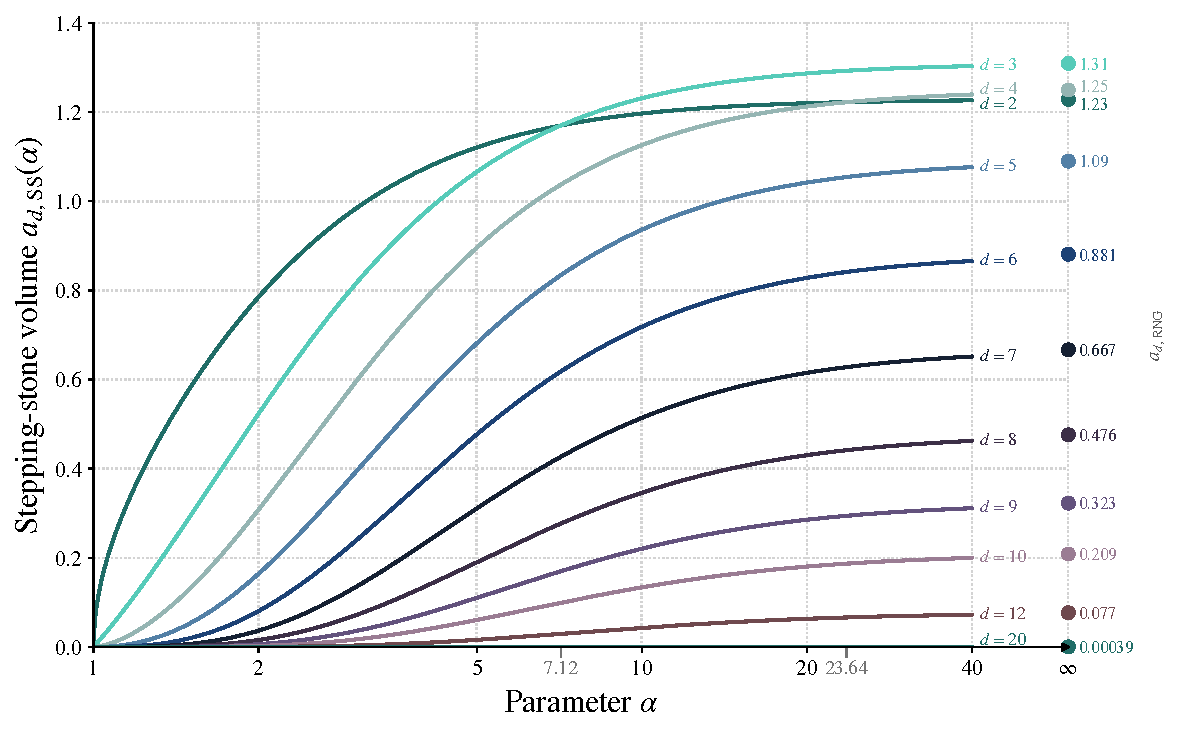
\includegraphics[width=1\linewidth]{stepping_stone_volume_log_scale.pdf}
    \caption{Numerical values of $a_{d,\mathrm{SS}}(\alpha)$ for several
    dimensions on a logarithmic $\alpha$-axis. The right endpoint shows
    $a_{d,\mathrm{RNG}}$, the relative-neighborhood limit. The auxiliary
    labels $7.12$ and $23.64$ mark the two numerical intersections described
    in the text.}
    \label{fig:ss-volume-curves}
\end{figure}
% \FloatBarrier

\subsection{Independent rejection-sampling validation}

The Monte Carlo calculation evaluates the original defining inequality in
\eqref{eq:unit-region}; it does not use the boundary parametrization or either
quadrature formula. 

The region is contained in the cylinder
\begin{equation}
    C_{d,\alpha}
    :=[0,1]\times B_{d-1}(0,r_\alpha),
    \qquad
    r_\alpha:=\sqrt{2^{-\nicefrac{2}{\alpha}}-\frac14}.
\end{equation}
Here $B_{d-1}(0,r_\alpha)$ denotes the closed ball of radius
$r_\alpha$ in $\R^{d-1}$.
Indeed, the defining inequality gives $0\leq X\leq1$. If $(X,Z)$ belongs to
the normalized region, midpoint symmetry in \Cref{prop:geometry} shows that
its reflection $(1-X,Z)$ also belongs to it; convexity then places their
midpoint $(\nicefrac{1}{2},Z)$ in the region. The largest
possible transverse norm is therefore attained in the midpoint slice, where
the defining equality gives $\norm{Z}=r_\alpha$. Consequently,
\begin{equation}
    V_{d,\alpha}:=\lambda_d(C_{d,\alpha})
    =\kappa_{d-1}r_\alpha^{d-1}.
\end{equation}
If $H$ of $N$ independent uniform points in this cylinder satisfy
\eqref{eq:unit-region}, then
\begin{equation}
\begin{aligned}
\widehat p
:&=\frac{H}{N},
\\
\widehat a^{\mathrm{MC}}
&=
V_{d,\alpha}\widehat p
=
V_{d,\alpha}\frac{H}{N},
\\
\widehat{\operatorname{se}}
&=
V_{d,\alpha}
\sqrt{
\frac{\widehat p(1-\widehat p)}{N}
}.
\end{aligned}
\end{equation}


Where \(\widehat a^{\mathrm{MC}}\) is the Monte Carlo estimate for
\(a_{d,\mathrm{SS}}(\alpha)\),
\(\widehat{\operatorname{se}}\) is the standard error of the Monte Carlo estimate,
and \(\widehat p\) is the proportion of points that fall in the region. 
Thus the estimator is unbiased, and its reported standard error is the usual
binomial plug-in estimate.

We evaluated 18 parameter combinations with $N=10^8$ samples each, for a
total of $1.8\times10^9$ membership tests. The parameters were
$\alpha=1.25$ and $10$ in dimensions 2, 3, 4, 5, 8, 9, 10, 12, and 20.
Each run used a recorded deterministic seed. The complete results are
reported in \Cref{tab:mc-validation}.

\begin{table*}[pos=htbp]
\centering
\caption{Monte Carlo validation of the stable quadrature formula. Each row
uses $10^8$ samples. Here
$\varepsilon_{\mathrm{rel}}=(\widehat a^{\mathrm{MC}}-a^{\mathrm{quad}})/
a^{\mathrm{quad}}$, and $z$ is the discrepancy divided by its Monte Carlo
standard error. The notation $x\mathrm{e}k$ denotes $x\times10^k$.}
\label{tab:mc-validation}
\begingroup
\scriptsize
\setlength{\tabcolsep}{2.15pt}
\renewcommand{\arraystretch}{1.08}
\begin{minipage}[t]{0.495\linewidth}
\centering
\begin{tabular}{@{}rrrrrr@{}}
\toprule
\multicolumn{6}{c}{$\alpha=1.25$}\\
\cmidrule(lr){1-6}
$d$ & $a^{\mathrm{quad}}$ & $\widehat a^{\mathrm{MC}}$ & s.e. &
$10^4\varepsilon_{\mathrm{rel}}$ & $z$\\
\midrule
 2 & 0.41429435 & 0.41431538 & $2.501\mathrm{e}{-5}$  &  0.508 &  0.841\\
 3 & 0.15209303 & 0.15209032 & $1.226\mathrm{e}{-5}$  & -0.178 & -0.221\\
 4 & 0.04995978 & 0.04995401 & $4.721\mathrm{e}{-6}$  & -1.156 & -1.223\\
 5 & 0.01493763 & 0.01493994 & $1.572\mathrm{e}{-6}$  &  1.546 &  1.469\\
 8 & $2.567962\mathrm{e}{-4}$ & $2.567629\mathrm{e}{-4}$ & $3.299\mathrm{e}{-8}$  & -1.297 & -1.009\\
 9 & $5.884669\mathrm{e}{-5}$ & $5.885745\mathrm{e}{-5}$ & $7.912\mathrm{e}{-9}$  &  1.827 &  1.359\\
10 & $1.283446\mathrm{e}{-5}$ & $1.283558\mathrm{e}{-5}$ & $1.795\mathrm{e}{-9}$  &  0.869 &  0.622\\
12 & $5.352895\mathrm{e}{-7}$ & $5.352658\mathrm{e}{-7}$ & $8.002\mathrm{e}{-11}$ & -0.443 & -0.297\\
20 & $4.188191\mathrm{e}{-13}$& $4.187867\mathrm{e}{-13}$& $7.450\mathrm{e}{-17}$ & -0.772 & -0.434\\
\bottomrule
\end{tabular}
\end{minipage}%
\hfill
\begin{minipage}[t]{0.495\linewidth}
\centering
\begin{tabular}{@{}rrrrrr@{}}
\toprule
\multicolumn{6}{c}{$\alpha=10$}\\
\cmidrule(lr){1-6}
$d$ & $a^{\mathrm{quad}}$ & $\widehat a^{\mathrm{MC}}$ & s.e. &
$10^4\varepsilon_{\mathrm{rel}}$ & $z$\\
\midrule
 2 & 1.1966680  & 1.1967769  & $6.732\mathrm{e}{-5}$ &  0.910 &  1.617\\
 3 & 1.2306930  & 1.2306571  & $9.406\mathrm{e}{-5}$ & -0.291 & -0.381\\
 4 & 1.1257499  & 1.1255807  & $1.019\mathrm{e}{-4}$ & -1.503 & -1.660\\
 5 & 0.93604703 & 0.93620155 & $9.501\mathrm{e}{-5}$ &  1.651 &  1.626\\
 8 & 0.34611889 & 0.34607030 & $4.336\mathrm{e}{-5}$ & -1.404 & -1.120\\
 9 & 0.22068237 & 0.22068795 & $2.900\mathrm{e}{-5}$ &  0.253 &  0.192\\
10 & 0.13394539 & 0.13397369 & $1.835\mathrm{e}{-5}$ &  2.113 &  1.542\\
12 & 0.04328974 & 0.04329731 & $6.355\mathrm{e}{-6}$ &  1.749 &  1.192\\
20 & $1.226485\mathrm{e}{-4}$ & $1.226420\mathrm{e}{-4}$ & $2.155\mathrm{e}{-8}$ & -0.527 & -0.300\\
\bottomrule
\end{tabular}
\end{minipage}
\endgroup
\end{table*}

All 18 theoretical values lie within the corresponding two-sided normal
95\% Monte Carlo intervals: the maximum absolute standardized discrepancy is
$1.660$, and the maximum absolute relative error is
$2.113\times10^{-4}$. The largest absolute quadrature error estimate reported
by the adaptive routine across these cases is $3.552\times10^{-11}$. 
These results provide numerical support for the theoretical predictions.  

% \section{Conclusion}
% \label{sec:conclusion}

% We determined the volume of the stepping-stone diversion neighborhood in
% \(\R^d\) for every \(d\geq2\). For two distinct sites \(p\) and
% \(q\), the volume factorizes as
% \begin{equation}
% \lambda_d\!\left(S_{\mathrm{SS},\alpha}(p,q)\right)
% =
% \norm{p-q}^d a_{d,\mathrm{SS}}(\alpha),
% \end{equation}
% where the normalized constant depends only on \(d\) and \(\alpha\).
% Using an explicit boundary parametrization and orthogonal cross-sections,
% we reduced the computation of $a_{d,\mathrm{SS}}(\alpha)$ to a
% one-dimensional integral valid for every $\alpha>1$.

% The formula recovers the degenerate and Gabriel region cases. At the other endpoint,
% we strengthen the previously recognized planar graph limit: in every
% dimension, the finite-parameter neighborhoods, after removal of the defining
% sites, increase from within to the open relative-neighborhood lune, and their
% volumes converge to Devroye's classical unit-lune constant.
% For each finite point set, the corresponding graph in fact stabilizes
% at the open-lune relative-neighborhood graph for a finite parameter.
% Strict region
% inclusion makes the graphs decrease under edge inclusion, places them between
% the relative-neighborhood and Gabriel graphs in the corresponding parameter
% ranges, and yields connectivity for every nonempty finite point set and
% every $\alpha\geq1$.
% The parameter \(\alpha=2\) is also the sharp threshold for guaranteed
% geometric and abstract planarity in dimension two. For \(\alpha\geq2\),
% Gabriel or Delaunay edges provide candidate sets, but these inclusions do
% not by themselves give a linear-time planar algorithm or a subquadratic
% higher-dimensional algorithm.

% Devroye's regular-set theorem identifies the limiting conditional
% expected degree in every dimension and yields a general asymptotic lower
% bound for the expected number of edges:
% \begin{equation}
%     \lim_{n\to\infty}
%     \E\!\left[N_n(X_1)\mid X_1=x\right]
%     =
%     \frac{\kappa_d}{a_{d,\mathrm{SS}}(\alpha)}.
% \end{equation}
% For planar graphs with
% $\alpha\geq2$, worst-case sparsity upgrades that bound to the exact limit
% $\nicefrac{\pi}{[2a_{2,\mathrm{SS}}(\alpha)]}$ under Devroye's density regularity
% condition.
% In Watanabe's planar homogeneous
% Poisson point process, it gives the corresponding graph-edge-length density
% \begin{equation}
%     2\rho a_{2,\mathrm{SS}}(\alpha)r
%     e^{-\rho a_{2,\mathrm{SS}}(\alpha)r^2},
% \end{equation}
% which specializes to Watanabe's Gabriel formula at $\alpha=2$ and approaches
% his relative-neighborhood formula as $\alpha\to\infty$.
% This calculation and the planar volume formula are planar
% specializations.
% The Delaunay containment itself, the general
% Devroye degree limit and edge-count lower bound, and the remaining geometric,
% analytic, and graph-theoretic results hold for every \(d\geq2\).

% A change of variables yields stable quadrature, independently validated by a
% rejection sampler applied to the original region inequality. Across 18 runs of
% $10^8$ samples, every discrepancy was below two Monte Carlo standard errors.
% Continuity and strict monotonicity additionally make the normalized
% volume, and hence the limiting expected degree, an invertible calibration of
% the diversion parameter.


\section{Conclusion}
\label{sec:conclusion}

We developed an arbitrary-dimensional geometric analysis
for the
stepping-stone diversion neighborhood. As proved in
\Cref{prop:factorization}, similarity normalization isolates a normalized
volume constant through \eqref{eq:volume-factorization}.

The boundary profile is explicitly parametrized in
\Cref{prop:boundary-parametrization}. Integrating its orthogonal
cross-sections then gives the one-dimensional representation
\eqref{eq:main-integral} of \Cref{thm:main}, valid for every
$d\geq2$ and every finite $\alpha>1$.

The resulting formula places three distinguished geometric regimes within
a single framework. By \Cref{prop:special-cases}, at $\alpha=1$ the
neighborhood degenerates to the segment joining the defining sites, whereas
at $\alpha=2$ it is the closed Gabriel ball. By
\Cref{prop:rng-limit}, as $\alpha\to\infty$ the finite-parameter
neighborhoods, after removal of their defining sites, converge from within
to the open relative-neighborhood lune, and their normalized volumes
converge to the relative-neighborhood-lune constant given in
\eqref{eq:rng-constant}.

The strict increase of the diversion neighborhoods and their normalized
volumes is established in \Cref{thm:monotonicity}. Together with
continuity, this yields the calibration result of
\Cref{cor:continuous-calibration}: the map
\begin{equation}
\alpha\longmapsto a_{d,\mathrm{SS}}(\alpha)
\end{equation}
is continuous and strictly increasing from $[1,\infty)$ onto
$[0,a_{d,\mathrm{RNG}})$. Consequently, every normalized volume strictly
between the degenerate and relative-neighborhood values determines a unique
finite diversion parameter.

At the graph level, \Cref{prop:inclusions} shows that enlargement of the
diversion neighborhood reverses edge inclusion and places the stepping-stone
graph family within the classical proximity-graph inclusion hierarchy. In particular, for every finite parameter value, the stepping-stone graph contains the open-lune
relative-neighborhood graph and therefore contains a Euclidean minimum
spanning tree. This yields connectivity for every nonempty finite point set
in every ambient dimension, as stated in \Cref{cor:graph-consequence}.
Furthermore, \Cref{cor:finite-stabilization} shows that, for every fixed
finite point set, the stepping-stone graph coincides exactly with the
open-lune relative-neighborhood graph once the diversion parameter exceeds
a finite threshold depending on that point set. Thus the graph does not
merely converge asymptotically: it eventually stabilizes exactly. As shown
in \Cref{rem:stabilization-threshold}, however, no single finite threshold
works uniformly over all finite point sets.

For $\alpha\geq2$, the inclusion chain in \eqref{eq:tail-chain} places the
stepping-stone graph inside the Gabriel and Delaunay graphs. In the plane
and under general position, this provides a linear-size Delaunay starting
graph, as used by
\citet{kannangara2018stepping,kannangara2019stepping}. It does not, by
itself, produce a linear-time construction, because testing every initial
edge against the remaining sites still gives a naive quadratic procedure.
In higher dimensions, the same containment does not even guarantee a
subquadratic worst-case starting set: Delaunay and Gabriel graphs can
already have quadratic size in three dimensions
\citep{agarwal1992relative,chazelle1994selecting}.

The regularity verification in \Cref{prop:devroye-regularity} permits the
application of Devroye's theorem 
for graphs defined by regular sets.
In particular,
\Cref{cor:devroye-degree} gives the limiting conditional expected degree
in \eqref{eq:devroye-degree} and the asymptotic edge-count lower bound in
\eqref{eq:devroye-edge-lower-bound}. These conclusions are applications of
Devroye's  ta{general results}; the new input supplied here is the explicit
stepping-stone volume constant in arbitrary dimension.

In the planar homogeneous Poisson setting,
\Cref{prop:poisson-edge-density} substitutes the normalized area into
Watanabe's edge-length formulation. The resulting edge-length density
is given in \eqref{eq:watanabe-density}. At $\alpha=2$, it specializes
to the Gabriel-graph edge-length density, whereas, as
$\alpha\to\infty$, it converges to 
relative-neighborhood-graph edge-length density.

Finally, the change of variables introduced in
\Cref{prop:stable-quadrature} removes the endpoint singularity and produces
the stable quadrature formula \eqref{eq:stable-ss-integral}. The calculation
is implemented in the \textsc{ProximityGraphs} Python package, as described
in \Cref{sec:implementation}, and is validated numerically by the
rejection-sampling experiments reported in \Cref{tab:mc-validation}. The
rejection sampler evaluates the original defining inequality and does not
use the boundary parametrization or either quadrature formula; its only
additional geometric input is the proved enclosing cylinder.

The principal outcome is therefore a dimension-uniform reduction from an
implicit Euclidean region to an explicit boundary profile and a computable
one-dimensional volume formula. This representation simultaneously explains
the special and limiting geometries, strict parameter dependence,
proximity-graph inclusions, random-graph constants, and stable numerical
evaluation. More broadly, this analysis motivates the study of other
empty-region graph families whose pairwise regions, for each fixed parameter
value, are obtained from a single normalized template by translation,
rotation, and scaling. 
Examples include the influence regions of $\beta$-skeletons
\citep{kirkpatrick1985framework} and the two-parameter regions defining
planar $\gamma$-neighborhood graphs \citep{veltkamp1992gamma}.
For such families, the normalized template
provides a natural starting point for investigating the geometry and volume
of the corresponding empty regions and their consequences for the associated
graphs.

\printcredits

\section*{Code and data availability}
No external datasets were used. The exact computational release is archived
on Zenodo under
\href{https://doi.org/10.5281/zenodo.21291269}{DOI
10.5281/zenodo.21291269}~\citep{espino2026computational}. It contains the
quadrature, Monte Carlo, and figure-generation code, outputs, random seeds, and
reproduction instructions. The
\href{https://github.com/heri-espino/Stepping-Stone-Volume-Constants}{public
GitHub repository} hosts the maintained version of these materials. To
complement \Cref{fig:ss-regions}, the same companion provides an
\href{https://heri-espino.github.io/Stepping-Stone-Volume-Constants/}{interactive
three-dimensional visualization} of the normalized diversion neighborhood;
the parameter $\alpha$ can be varied continuously, and the region can be
rotated and magnified. Two supplementary CSV files underlying
\Cref{tab:mc-validation} add the hit counts, acceptance rates, sampling-cylinder
volumes, quadrature error estimates, sample counts, and random seeds for each
run.



    The reusable Python implementation is available in the
\href{https://pypi.org/project/proximitygraphs/}{\textsc{ProximityGraphs}
package on PyPI} and in its
\href{https://github.com/HectorMaravillo/ProximityGraphs}{public source
repository}; the version used here is archived under
\href{https://doi.org/10.5281/zenodo.21088183}{DOI
10.5281/zenodo.21088183}~\citep{maravillo2026proximitygraphs}.


\section*{Declaration of competing interest}
The authors declare no competing interests.

\section*{Declaration of generative AI and AI-assisted technologies in the manuscript preparation process}
During the preparation of this work, the authors used ChatGPT by OpenAI to
assist with language, clarity, organization, and LaTeX formatting. After
using this tool, the authors reviewed and edited the content as needed and
take full responsibility for the content of the publication.

\section*{Funding}
This research did not receive any specific grant from funding agencies in the public, commercial, or not-for-profit sectors.

\bibliographystyle{cas-model2-names}
\bibliography{references}

\end{document}
